\partimage[width=1\columnwidth]{Figures/PartImages/FigCh4.png}
\part{Polarisation circulaire, molécules chirales et harmoniques d'ordre élevé}
\label{PA:Spin_HHG}
\chapter{Génération d'harmoniques d'ordre élevé polarisées elliptiquement}
\label{CH:Circular_HHG}
Dans cette partie nous présenterons comment générer des harmoniques d'ordre élevé portant du moment angulaire de spin, c'est-à-dire ayant une polarisation elliptique. Pour commencer nous donnerons le formalisme utile à la description d'ondes polarisées, puis étudierons le mécanisme de GHOE dans un atome ou une molécule quand le laser de génération est polarisé elliptiquement. Nous verrons que le transfert de moment angulaire n'est pas efficace dans le schéma habituel de GHOE et mentionnerons les solutions existantes, avant d'en démontrer une nouvelle qui utilise une résonance de l'atome ou la molécule de génération.

\section{Formalisme pour la description d'ondes polarisées elliptiquement}
\label{sec:polardef}
Comme on l'a vu dans la partie \ref{sec:circpolar}, le champ électrique d'une onde polarisée elliptiquement décrit une ellipse au cours de sa propagation. Soit $(x,y,z)$ un repère cartésien tel que $z$ soit selon la direction de propagation et $x$ soit selon l'axe majeur de l'ellipse. Un champ elliptique monochromatique s'écrit :
\begin{equation}
\bm{E}=\begin{pmatrix}
E_{x}\cos{(\omega t-kz)}\\
E_{y}\sin{(\omega t-kz)}\\
0
\end{pmatrix}=E_{0}
\begin{pmatrix}
\cos{(\omega t-kz)}\\
\epsilon\sin{(\omega t-kz)}\\
0
\end{pmatrix},
\label{eq:jones}
\end{equation}
où $\epsilon = E_{y}/E_{x}$ est appelé ellipticité du champ. $\epsilon$ varie de 0 pour une polarisation linéaire à 1 pour une polarisation circulaire.  On a vu que si $\epsilon>0$ (resp. $<0$), l'onde était elliptique gauche (resp. droite) et porte un moment angulaire de spin de $\epsilon\hbar$ (resp. $-\epsilon\hbar$) par photon. 

\begin{figure}[!ht]
\centering
\def\svgwidth{0.6\columnwidth}
\import{Figures/Polar/}{polarellipse.pdf_tex}
\caption{Définition des différents paramètres de l'ellipse de polarisation.}
\label{Fig:polarellipse}
\end{figure}
Dans un repère où $x$ et $y$ ne sont pas selon les axes de l'ellipse, on note $\eta$ l'angle entre l'axe $x$ et l'axe majeur de l'ellipse (voir figure \ref{Fig:polarellipse}). L'ellipticité est déterminée par le rapport des axes mineurs et majeurs de l'ellipse, $b$ et $a$ : $\epsilon = b/a$. On note $\chi$ l'angle tel que $\tan\chi = \epsilon = b/a$. Comme les amplitudes du champ selon les axes de l'ellipse sont déphasées de $\pi/2$, $a$ et $b$ peuvent être vus comme les parties réelle et imaginaire d'un vecteur de polarisation complexe et unitaire $\bm{\Pi}$. Le champ s'écrit alors :
\[\bm{E} = E_x \bm{e_x} + E_y \bm{e_y} = E_0(\Pi_x \bm{e_x} + \Pi_y \bm{e_y}).\] 
Il sera utile d'utiliser les \textit{paramètres de Stokes}, définis comme :
\begin{align}
s_0 &= E_xE_x^*+E_yE_y^* =E_0^2,\nonumber\\
s_1 &= E_xE_x^*-E_yE_y^* =E_0^2\cos 2\chi\cos 2\eta ,\nonumber\\
s_2 &= -\left(E_xE_y^*+E_yE_x^*\right)=E_0^2\cos 2\chi\sin 2\eta,\nonumber\\
s_3 &= -\rmi\left(E_xE_y^*-E_yE_x^*\right)=E_0^2\sin 2\chi,	
\label{eq:stokes1}
\end{align}
où nous avons utilisés les conventions de signe de \mycite{barron}. Pour une onde monochromatique, ces paramètres donnent $E_0$, $\chi$ et $\eta$, ou de manière équivalente, l'intensité $I_0$, l'ellipticité $\epsilon$ et $\eta$. Ils caractérisent donc totalement le champ électrique. Il ne sont pas indépendants : on a $s_0^2 = s_1^2+s_2^2+s_3^2$. 

En pratique, les ondes utilisées ne sont que \textit{quasi}-monochromatiques. Elles possèdent une largeur spectrale $\Delta\omega$ non nulle, à l'intérieur de laquelle les différentes composantes fréquentielles ne possèdent pas forcément les mêmes polarisations et phases. Le vecteur du champ électrique apparent, somme de toutes les composantes fréquentielles, ne décrit alors plus une ellipse. Dans le cas extrême, il ne présente aucune direction préférentielle : on parle alors de lumière \textit{non polarisée}. De manière générale, le vecteur du champ électrique n'évolue pas complètement régulièrement ou irrégulièrement, la lumière est alors dite \textit{partiellement} polarisée.

Dans une expérience, le temps d'observation est en général long comparé à $1/\Delta\omega$. Les paramètres de Stokes doivent donc être définis à partir de la moyenne temporelle des quantités définies en \ref{eq:stokes1}. Ces expressions font intervenir les produits des composantes de $\bm{\Pi}$. Pour une lumière complètement polarisée,
\[\overline{\Pi_x \Pi^*_y} = \Pi_x \Pi^*_y,\]
et on retrouve les mêmes propriétés que pour une onde monochromatique. \`{A} l'autre extrême, si la lumière est non polarisée, toutes les orientations de $\bm{\Pi}$ sont équiprobables :
\[\overline{\Pi_x \Pi^*_y} = 0.\]
Les paramètres de Stokes deviennent donc $S_0 = E_0^2$ et $s_1^2 = s_2^2 = s_3^2 = 0$. Dans le cas d'une lumière partiellement polarisée, on obtient donc $s_0^2 > s_1^2+s_2^2+s_3^2$. On introduit alors le degré de polarisation de la lumière $P$, défini comme 
\[P = \frac{\sqrt{s_1^2+s_2^2+s_3^2}}{s_0}.\] $P$ varie entre $0$ pour une lumière non polarisée et $1$ pour une polarisation complète. Une lumière partiellement polarisée peut être séparée entre une composante non polarisée et une complètement polarisée, dont les paramètres d'ellipse sont bien définis. On les retrouve à partir des paramètres de Stokes :
\begin{align}
s_0 &= E_0^2,\nonumber\\
s_1 &= PE_0^2\cos 2\chi\cos 2\eta ,\nonumber\\
s_2 &= PE_0^2\cos 2\chi\sin 2\eta,\nonumber\\
s_3 &= PE_0^2\sin 2\chi,	
\label{eq:stokes2}
\end{align}
Les paramètres de l'onde s'obtiennent en inversant \ref{eq:stokes2} :
\begin{align}
E_0^2 &= s_0,\nonumber\\
\eta &= \frac{1}{2} \arctan\left(\frac{s_2}{s_1}\right),\nonumber\\
\chi &= \frac{1}{2} \arctan\left(\frac{s_3}{\sqrt{s_1^2+s_2^2}}\right),\nonumber\\
P &= \sqrt{s_1^2+s_2^2+s_3^2}/s_0
\label{eq:stokes2inv}
\end{align}

L'onde est maintenant complètement décrite par $E_0$, $\chi$, $\eta$ et $P$. Cette description est similaire à celle d'un système en mécanique quantique. En effet, une description vectorielle telle que l'expression \ref{eq:jones} (appelé vecteur de Jones) ne peut décrire qu'une polarisation complète. Une polarisation partielle est une superposition incohérente de polarisations complètes, bien décrite par le formalisme de Stokes. De la même manière, un état quantique pur est décrit par une fonction d'onde, analogue du vecteur de Jones. Un état quantique mixte, qui est une superposition d'états purs, doit être décrit par une matrice densité, analogue du vecteur de Stokes. Cette analogie n'est pas fortuite : la lumière provient généralement d'une transition entre deux états quantiques, par exemple d'un atome. Les propriétés de polarisation de la lumière découlent alors de la cohérence entre ces états, comme décrit en détail dans \mycite{fano1957}. 

Pour terminer, notons qu'en plus d'une inhomogénéité temporelle, la polarisation partielle de la lumière peut également découler d'une inhomogénéité spatiale : si les paramètres de l'ellipse varient avec la coordonnée transverse et que l'expérience moyenne spatialement ces différentes contributions, on aura $P<1$.

\section{GHOE à partir d'un faisceau infrarouge polarisé elliptiquement}
\label{sec:ghoepolar}
Dans la partie précédente, nous avons démontré qu'en donnant du moment angulaire orbital à l'infrarouge de génération, il était transmis au rayonnement harmonique. Ce principe devrait s'appliquer au moment angulaire de spin, qui doit être conservé dans le processus. 

\subsection{Résultats de la littérature}
\mycite{budilPRA1993} ont réalisé la première expérience à ce sujet. Ils ont généré les harmoniques d'ordre élevé d'un laser Cr:LiSAF et mesuré l'intensité de chaque harmonique en fonction de l'ellipticité de l'infrarouge. Le résultat pour le néon est présenté sur la figure \ref{Fig:budil}.
\begin{figure}[!ht]
\centering
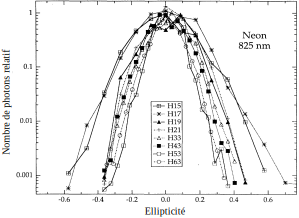
\includegraphics[width=0.6\columnwidth]{Figures/Polar/Intensity_f_ellipticity_budil}%
\caption{Intensité normalisée des harmoniques produites dans le néon en fonction de l'ellipticité. Tiré de \mycite{budilPRA1993}}%
\label{Fig:budil}%
\end{figure}

On observe une décroissance de l'intensité harmonique en fonction de l'ellipticité. Cet effet est marqué : on perd environ un ordre de grandeur en intensité quand $|\epsilon_{IR}| = 0.2$. On remarque également que cette décroissance est de plus en plus piquée lorsque l'ordre harmonique augmente.

\'{E}tudions ensuite les résultats de \mycite{AntoinePRA1997}. Les auteurs se sont cette fois intéressés à l'état de polarisation du rayonnement harmonique en fonction de l'ellipticité de l'infrarouge. Ces expériences ont été réalisées sur une version antérieure du système laser que nous avons utilisé dans la partie III. Pour caractériser le rayonnement, les auteurs mesurent des \textit{lois de Malus}, méthode optique qui sera présentée plus loin (section \ref{sec:resonant_argon_exp}). Comme on le verra, cette technique est incapable de mesurer le degré de polarisation $P$. Elle ne donne qu'une borne supérieure sur l'ellipticité, atteinte uniquement lorsque la lumière est complètement polarisée. Ce point est crucial dans le cas de la GHOE : comme expliqué dans la partie \ref{sec:phase_spatiale} le dipôle de chaque ordre harmonique dépend de l'intensité infrarouge. Le champ émis sera donc non homogène en polarisation spatialement et temporellement, donc nécessairement partiellement polarisé.

La figure \ref{fig:antoinepra} présente quelques résultats extraits de \mycite{AntoinePRA1997}. On y voit l'évolution de l'ellipticité des harmoniques et de l'angle d'orientation de l'ellipse $\eta$, pris par rapport à un axe de référence fixe. L'ellipticité mesurée n'étant qu'une borne supérieure de l'ellipticité vraie, on la note $\epsilon^{max}_q$. La figure \ref{fig:antoinepra} inclut un résultat numérique qui donne lui accès à $P$ et donne une idée de la quantité de lumière non-polarisée.

\begin{figure}[!ht]
\centering
\def\svgwidth{\columnwidth}
\import{Figures/Polar/}{antoinePRA.pdf_tex}
\caption{\`{A} gauche, mesure de l'ellipticité des harmoniques 17 et 23 générées dans l'argon par un champ infrarouge elliptique. Carrés rouges : mesures expérimentales de $\epsilon^{max}_q$ par loi de Malus. Comme expliqué plus haut, ce n'est qu'une borne supérieure sur la vraie valeur de l'ellipticité. En traits rouges, même quantité obtenue par le calcul. En pointillés noirs, véritable ellipticité obtenue par le calcul. En traits-pointillés verts, degré de polarisation obtenu par le calcul. \`{A} droite, mesure de l'angle de rotation de l'ellipse (carrés rouges) et même quantité obtenue par le calcul (traits rouges). Adapté de \mycite{AntoinePRA1997}.}
\label{fig:antoinepra}
\end{figure}

On fait les observations suivantes :
\begin{itemize}
\renewcommand{\labelitemi}{$\bullet$}
\setlength\itemsep{1em}
\item $\epsilon^{max}_q$ est une fonction croissante de $\epsilon_{IR}$ sur l'intervalle parcouru.
\item $|\epsilon^{max}_q|$ augmente plus rapidement avec $|\epsilon_{IR}|$ pour l'harmonique plus basse.
\item Le rayonnement est de moins en moins polarisé à mesure que $|\epsilon_{IR}|$ augmente. Cet effet est plus fort pour l'harmonique basse.
\item Cette diminution de $P$ s'accompagne d'une ellipticité vraie plus faible. Pour l'harmonique la plus basse, l'ellipticité vraie est presque \textit{deux fois inférieure} à l'ellipticité mesurée.
\item $\eta$ est également une fonction croissante de $\epsilon_{IR}$.
\item $\eta$ augmente plus rapidement pour l'harmonique basse.
\end{itemize}
\vspace{\baselineskip}
Ces deux travaux démontrent deux résultats généraux. En premier lieu, on voit que l'ellipticité de l'infrarouge est bien transférée au champ harmonique. Toutefois, l'ellipticité harmonique semble toujours rester inférieure à celle du laser générateur. Deuxièmement, le rendement harmonique décroît exponentiellement avec l'ellipticité de l'infrarouge. Nous concluons donc qu'il est très difficile d'obtenir un rayonnement ultraviolet d'ellipticité significative tout en gardant un niveau de signal suffisant. Dans la section suivante, nous expliquons les effets physiques à l'origine de ces propriétés.

\subsection{Description théorique de la GHOE en polarisation elliptique}
Dans le modèle à trois étapes (voir section \ref{sec:threestep}), la polarisation du champ intervient dans le calcul de la trajectoire électronique dans le continuum. On note $(x,y)$ la position dans le plan transverse de l'électron, que l'on considère classiquement. Sa trajectoire dans un champ complètement polarisé est donnée par :
\[\left\{
\begin{array}{l}
  \ddot{x}(t) = -\frac{qE_0}{m}\cos\omega t \\
  \ddot{y}(t) = -\epsilon\frac{qE_0}{m}\sin\omega t,
\end{array}
\right.\]
avec $q$ et $m$ la charge et la masse de l'électron, et $\epsilon$ et $\omega$ l'ellipticité et la fréquence angulaire du champ. L'équation selon $x$ se résoud exactement de la même façon que pour une polarisation linéaire : on suppose $x(t_i) = \dot{x}(t_i) = 0$, où $t_i$ est le temps d'ionisation, et pour chaque $t_i$, on obtient l'instant de recombinaison $t_r$.

Selon la dimension $y$, l'électron doit bien sûr être émis au niveau du noyau : $y(t_i) = 0$. Cependant, si on suppose que $\dot{y}(t_i) = 0$, l'équation $y(t_r) = 0$ n'a pas de solution : l'électron 'rate' l'atome et ne peut pas recombiner, comme illustré sur la figure \ref{fig:ellgruson}.

\begin{figure}[!ht]
\centering
\def\svgwidth{0.7\columnwidth}
\import{Figures/Polar/}{trajClassique.pdf_tex}
\caption{Trajectoire classique d'un électron dans un champ électrique elliptique, en supposant $x(t_i) = \dot{x}(t_i) = 0$ et $y(t_i) = \dot{y}(t_i) = 0$. La longueur d'onde est 800 nm et l'éclairement est $\SI{2e14}{W/cm^2}$. La polarisation du champ infrarouge est schématisée en gris. Adapté de \mycite{gruson}.}
\label{fig:ellgruson}
\end{figure}

Classiquement, la génération d'harmonique en polarisation elliptique est donc impossible. En vérité, le déplacement et la vitesse de l'électron selon l'axe $y$ sont trop faibles pour utiliser une description classique. Si on décrit cette dimension quantiquement, on a un paquet d'onde électronique émis lors de l'ionisation tunnel. Ce paquet d'onde est localisé spatialement autour de l'atome, sur une longueur $\Delta y$ dépendant de l'orbitale en jeu. Le moment cinétique selon $y$ est donc lui aussi confiné à une largeur $\Delta p_y$. La distribution de $p_y$ est centrée sur y=0 à $t=0$ et peut maintenant contenir des valeurs non nulles. \mycite{strelkov2006} démontre que pour avoir recombinaison, le moment cinétique initial doit valoir $p_y(t=0) = -\bar{y}/\tau$, où $\bar{y}$ est la quantité représentée sur la figure \ref{fig:ellgruson}, et $\tau$ le temps d'excursion total de l'électron. Ceci permet d'expliquer simplement le résultat de \mycite{budilPRA1993} présenté plus haut : si $\epsilon_{IR}$ augmente, $\bar{y}$ augmente également. Il faut donc un moment cinétique initial plus important pour avoir recombinaison, ce qui est moins probable puisque la distribution de $p_y(t=0)$ est centrée en y=0. Ceci explique la diminution du rendement harmonique avec l'ellipticité de l'infrarouge.

Pour comprendre qualitativement les résultats de \mycite{AntoinePRA1997}, on trace les trajectoires classiques de l'électron, cette fois avec la condition initiale $p_y(t=0) = -\bar{y}/\tau$ et avec les deux trajectoires quantiques.

\begin{figure}[!ht]
\centering
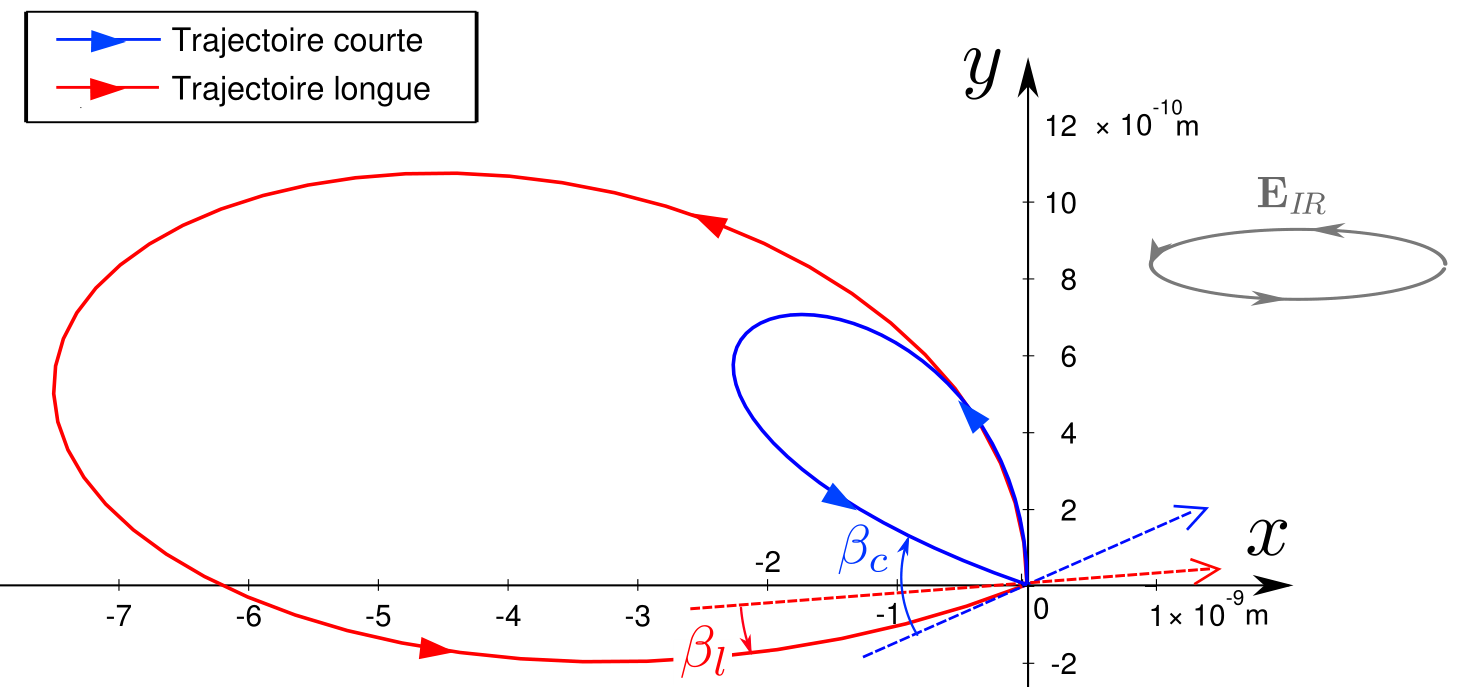
\includegraphics[width=0.9\columnwidth]{Figures/Polar/higuet.png}%
\caption{Trajectoires électroniques correspondant à l’harmonique 111 d'un laser à 1800 nm, pour un éclairement de $\SI{1e14}{W/cm^2}$ et une ellipticité de 0.2 (champ représenté en gris).
En ligne pointillée, la direction du champ à l’instant d’ionisation. On notera la différence entre les échelles
des axes $x$ et $y$. Tiré de \mycite{higuet}}
\label{fig:ellhiguet}%
\end{figure}

La figure \ref{fig:ellhiguet}, tirée de \mycite{higuet}, n'est pas directement comparable à la figure \ref{fig:ellgruson}, le calcul ayant été réalisé à une longueur d'onde plus élevée. Une longueur d'onde plus grande conduit à des trajectoires électroniques plus longues et à des effets plus marqués qu'à 800 nm.
On observe toutefois un effet intéressant : l'électron recombine sur l'atome avec un angle variable $\beta_{c/l}$ (pour trajectoire courte/longue). Cette angle est responsable de la rotation d'angle $\eta$ de l'ellipse harmonique. En effet, pour une orbitale de symétrie sphérique, l'axe principal de l'ellipse de polarisation du rayonnement harmonique est dirigé selon la direction de recollision de l'électron à la recombinaison \mycite{strelkov2006}. L'ellipse harmonique est donc tournée d'un angle $\beta_{c/l}\approx\eta$, qui dépend de l'ordre harmonique et de la trajectoire considérée. On remarque que $\beta_c$ et $\beta_l$ sont de signes différents, la dépendance de $\eta$ est donc de signe opposé pour la trajectoire longue. Ceci peut être mesuré expérimentalement (voir e.g. la figure 3.11 de \mycite{higuet}).\par
Enfin, cet angle explique également que le rayonnement harmonique soit elliptique. L'argument donné par \mycite{Strelkov2011} est le suivant : on considère un état lié $\psi_0(x,y,z) = \psi(x)\psi(y)\psi(z)$ et un paquet d'onde électronique. Ce paquet se déplace principalement dans la direction $x$ et possède une amplitude dans les deux autres dimensions : $\chi(x,y,z) = f(y,z)\exp(\rmi p_x x)$. Comme on l'a vu, l'amplitude $f(y,z)$ est initialement centrée en $y=0$ puis se décale selon $y$ au cours de la propagation. \`{A} la recombinaison, on peut faire un développement de Taylor de $f$ : $f(y,z) = f_0 + f_1 y$, où $f_1$ est relié à l'angle de recombinaison. Le moment dipolaire du système vaut 
\[\bm{d} = \int{\psi_0^* \bm{r} \chi \rmd\bm{r}} + \text{c.c.}\]
On obtient donc ses composantes cartésiennes :
\[d_x \propto f_0 \text{  et  } d_y \propto \rmi f_1.\]
On excite donc un dipôle dans les deux directions transverses, et leurs oscillations sont décalées de $\pi/2$. Le signal émis est donc polarisé elliptiquement.

\section{Méthodes existantes de génération d'harmoniques elliptiques}
Dans la partie précédente, nous avons expliqué le mécanisme de GHOE en polarisation elliptique et vu que le processus ne permettait pas un transfert direct et efficace de l'ellipticité de l'infrarouge vers l'ultraviolet. Nous présentons ici trois méthodes existantes pour circonvenir à ce problème. 

\subsection{Réflexion sur des surfaces métalliques}
\label{sec:metalsurface}
L'idée est ici de générer des harmoniques polarisée linéairement puis d'utiliser un dispositif similaire à une lame quart d'onde. Dans ces gammes spectrales, il est impossible de réaliser une lame quart-d'onde conventionnelle, mais on peut obtenir le même effet à partir de plusieurs surfaces métalliques. \par
On appelle plan d'incidence le plan formé par le vecteur d'onde du champ incident et le vecteur normal à la surface. Il est alors courant d'appeler $p$ la composante du champ \textit{parallèle} à ce plan et $s$ la composante perpendiculaire (\textit{senkrecht} en allemand). Selon le métal utilisé, ces deux composantes ne sont pas réfléchies également : la surface métallique présente une réflectivité selon chaque dimension, habituellement notées $R_p$ et $R_s$. De plus, elle introduit un déphasage entre ces deux composantes. Il est ainsi possible d'introduire un déphasage de $\pi/2$ en choisissant une bonne combinaison de miroirs. \mycite{VodungboOE2011} ont développé un dispositif à 4 miroirs de Mo/$\text{B}_\text{4}$C qui permettent d'obtenir les harmoniques 31 à 45 avec une ellipticité variant de 1 à 0.61. Ces caractéristiques sont très intéressantes, malgré un inconvénient majeur : la transmission du dispositif varie entre 2.6 et 3.7 \% sur la plage considérée. Ce type de dispositif a continué à être amélioré, \mycite{WillemsPRB2015} reportent par exemple une transmission de 10-30\% et une ellipticité de $\approx 0.8$ entre 45 et 70 eV.\par

Ces dispositifs sont assez difficiles à implémenter, ce qui couplé à leur faible transmission explique qu'ils ne soient pas très répandus aujourd'hui. 

\subsection{Génération dans des molécules alignées}
Considérons la GHOE avec un faisceau polarisé linéairement, cette fois dans un gaz de molécules diatomiques. Au niveau microscopique, l'orientation de l'axe de la molécule par rapport à la polarisation du laser joue un rôle crucial : l'angle de recombinaison de l'électron par rapport à cet axe modifie l'émission, exactement comme le champ elliptique représenté sur la figure \ref{fig:ellhiguet}. L'électron peut donc exciter les deux composantes du dipôle. L'interprétation est toutefois plus compliquée, puisque l'ellipticité obtenue dépend de la symétrie de ou des orbitales ionisées, de leur phases relatives ou encore de l'intensité de génération (voir \mycite{MairessePRL2010}). \par
\`{A} l'échelle macroscopique, toutes les orientations de molécules par rapport au laser sont équiprobables. On a donc un effet de moyenne, qui donne un rayonnement harmonique macroscopique polarisé linéairement. Il faut donc \textit{aligner} les molécules. Une technique courante est l'alignement impulsionnel, qui utilise une pré-impulsion quelques secondes avant l'impulsion de génération \mycite{RoscaPRL2001}. La figure \ref{fig:n2ell} présente deux exemples de résultats obtenus avec $\text{N}_\text{2}$, tirés de \mycite{ZhouPRL2009} et \mycite{MairessePRL2010}. Dans les deux cas, on observe un maximum d'ellipticité pour l'harmonique 23 et pour un angle d'alignement d'environ 60\degres.

\begin{figure}[!ht]
\centering
\def\svgwidth{1\columnwidth}
\import{Figures/Polar/}{n2ell.pdf_tex}
\caption{Mesures d'ellipticité en fonction de l'ordre harmonique et de l'angle d'alignement des molécules de $\text{N}_\text{2}$ par rapport à la polarisation du laser. \`{A} gauche, résultat tiré de \mycite{ZhouPRL2009}, où I = $\SI{2e14}{W/cm^2}$. \`{A} droite, résultat tiré de \mycite{MairessePRL2010}, où I = $\SI{8e13}{W/cm^2}$. Les ellipticités mesurées ici sont des bornes supérieures et non pas la vraie valeur.}
\label{fig:n2ell}
\end{figure}

Ce résultat s'explique en fait par la présence de plusieurs canaux d'ionisation et est donc très intéressant du point de vue de la spectroscopie harmonique. Il est toutefois assez peu flexible et nécessite d'aligner des molécules, et fournit une ellipticité modeste. De plus, l'utilisation d'une impulsion d'alignement a tendance à créer davantage d'inhomogénéités spatiales et temporelles, ce qui produit un rayonnement peu polarisé. Cette question est étudiée en détail expérimentalement dans la thèse de Vincent Gruson \mycite{gruson}.

\subsection{Manipulation de la trajectoire électronique par un champ bicolore}
Terminons par la méthode la plus récente, qui est peut-être la plus intuitive. Le principe est ici de contrôler optiquement la trajectoire électronique de sorte à ce que la recombinaison soit possible quelque soit l'ellipticité infrarouge. Une solution à ce problème a été initialement donnée par \mycite{EichmannPRA1995}. En utilisant un champ à deux couleurs d’ellipticités opposées et de deux longueurs d'onde commensurables, par exemple 400 et 800 nm, la GHOE est possible. L'expérience réalisée par \mycite{FleischerNP2014} montre que la génération est efficace dans ces conditions, et permet de générer des harmoniques paires et impaires d'ellipticité $|\epsilon^{max}_q|\approx 1$. \mycite{KfirNP2015} a mesuré l'hélicité (le signe de $\epsilon$) et montré que les ordres harmoniques étaient polarisés ainsi:
\[\left\{
\begin{aligned}
  \text{Si }q&=3m-1,\quad &\epsilon_q \approx \pm 1 \\
	&=3m+1, &\epsilon_q \approx \mp 1 \\
	&=3m, &\text{l'harmonique n'est pas générée},
\end{aligned}
\right.\]
où $\pm$ dépend de l'hélicité des champs générateurs. Cette méthode est très intéressante car elle produit un rayonnement fortement polarisé et intense. Elle a été utilisée avec succès par \mycite{KfirNP2015} pour réaliser des mesures de dichroïsme circulaire magnétique dans le cobalt, un effet voisin de ceux dont il sera question au chapitre \ref{sec:PECD}. Cette méthode est ainsi particulièrement adaptée à la spectroscopie de la phase solide.\par
La réponse d'une molécule est quant à elle plus difficile à interpréter. En effet, un grand nombre de degrés de liberté et différents canaux d'ionisation contribuent au spectre total, et il n'est jamais facile d'identifier chacune de ces contributions. 
On préférera donc avoir un rayonnement très simple, de sorte à exciter le moins d'effets possibles et de pouvoir les identifier. La technique présentée ici fournit un spectre harmonique dense fait d'harmoniques paires et impaires d'hélicité en alternance, ce qui est à l'opposé des besoins de la spectroscopie moléculaire.

\section{Une image photonique de la GHOE en polarisation elliptique}
Les travaux de \mycite{FleischerNP2014} que nous venons de mentionner ont suscité de nombreuses questions sur la conservation du moment angulaire de spin dans la GHOE. Avant ces travaux, la conservation du spin n'avait été étudiée ni théoriquement, ni expérimentalement.

Jusqu'à présent, nous avons utilisé une description macroscopique du champ électromagnétique. \`A l'étape de recombinaison de la GHOE, l'électron recombine sur l'état fondamental de l'atome. Le processus de GHOE peut être vu comme un processus \textit{paramétrique} dans lequel l'état initial et final sont les mêmes. On considère alors que chaque photon harmonique est issu de l'absorption et/ou de l'émission d'un certain nombre de photons du fondamental. Si la GHOE est effectivement un processus paramétrique, elle doit conserver l'énergie, la quantité de mouvement et les moments angulaires orbitaux et de spin. Nous avons pu observer la conservation des trois premières quantités au cours de cette thèse, et nous intéressons ici à la quatrième.

\mycite{FleischerNP2014} ont proposé un modèle simple prédisant le MAS de chaque harmonique dans leur dispositif à deux couleurs, en supposant la conservation du MAS. De manière surprenante, ils observèrent de très larges déviations à ce modèle et proposèrent deux mécanismes pour les expliquer : (1) l'électron ionisé emporte avec lui un moment angulaire de spin non nul, ce qui remet en question le fait que la GHOE soit un processus paramétrique, et (2) les différentes harmoniques sont émises de façon corrélées, ce qui empêche de considérer le moment angulaire de spin d'une harmonique seule.\par
\mycite{PisantyPRA2014} proposa ensuite un modèle différent, qui montra que les données de \mycite{FleischerNP2014} étaient cohérentes avec la conservation du MAS sans avoir à utiliser de tels arguments. Nous reprenons sa démarche pour expliquer le cas plus simple de la génération à un seul faisceau polarisé elliptiquement, déjà décrit macroscopiquement dans la partie \ref{sec:ghoepolar}, mais cette fois avec une image photonique.

On considère un champ d'ellipticité $\epsilon_0$ arbitraire. On décompose ce champ sur la base des ondes circulaires droites et gauches :
\begin{equation}
\bm{E} = \frac{E_0 e^{-\rmi\omega t}}{2\sqrt{2}}\left(\frac{1+\epsilon_0}{\sqrt{1+\epsilon_0^2}}\bm{e}_R+\frac{1-\epsilon_0}{\sqrt{1+\epsilon_0^2}}\bm{e}_L\right)+\text{c.c.},
\label{eq:Eell_RL}
\end{equation}
où $\bm{e}_{R/L}=(\bm{e}_x\pm\rmi\bm{e}_y)/\sqrt{2}$ sont les vecteurs unitaires complexes des polarisations circulaires droites et gauches.

Les composantes R et L du champ sont alors considérées séparément : on note $n_R$ et $n_L$ le nombre de photons respectif impliqués dans le processus. On note $q$ l'ordre harmonique, et la conservation de l'énergie s'écrit :
\[ q\hbar\omega = n_R\hbar\omega+n_L\hbar\omega, \]
soit $q = n_R + n_L$, ce qui est consistant avec la conservation de la parité car le nombre de photon absorbé est impair. On a donc un grand nombre de paires $(n_R,n_L)$ qui contribuent à l'émission de chaque harmonique $q$. On peut restreindre ces paires en écrivant la conservation du moment angulaire de spin pour chacune d'entre elles. En notant $s$ le MAS, on a :
\[s_{(n_R,n_L)} = n_R s_R + n_L s_L = n_R - n_L.\]
Le MAS d'un photon ne peut prendre que deux valeurs : $s_{(n_R,n_L)}=\pm1$, ce qui restreint les canaux possibles à 2 :
\[n_R = \frac{q+1}{2},\; n_L = \frac{q-1}{2}\quad\text{ou}\quad n_R = \frac{q-1}{2},\; n_L = \frac{q+1}{2}.\]

Ces deux canaux n'ont pas la même amplitude. Par simplicité, on suppose que l'amplitude d'un processus à n-photons évolue comme la $\text{n}^{i\`{e}me}$ puissance du champ fondamental. Cette approximation est un développement perturbatif à l'ordre le plus bas, qui a de nombreuses limitations pour la description de la GHOE, comme l'absence de plateau. On verra qu'elle permet toutefois de comprendre les comportements observés. Dans cette approximation, l'expression \ref{eq:Eell_RL} donne l'amplitude de chaque canal :
\[ E_{(n_R,n_L)} \propto \left(\frac{1+\epsilon_0}{\sqrt{1+\epsilon_0^2}}\right)^{n_R}\left(\frac{1-\epsilon_0}{\sqrt{1+\epsilon_0^2}}\right)^{n_L}\]
donc son intensité est :
\[ I_{(n_R,n_L)} \propto \left(\frac{1+\epsilon_0}{\sqrt{1+\epsilon_0^2}}\right)^{2n_R}\left(\frac{1-\epsilon_0}{\sqrt{1+\epsilon_0^2}}\right)^{2n_L}\]

On somme alors les deux canaux pondérés par $I_{(n_R,n_L)}$ pour obtenir la valeur moyenne du MAS de chaque harmonique :
\begin{align}
<s_q> &= \frac{I_{(\frac{q+1}{2},\frac{q-1}{2})} s_{(\frac{q+1}{2},\frac{q-1}{2})}+I_{(\frac{q-1}{2},\frac{q+1}{2})} s_{(\frac{q-1}{2},\frac{q+1}{2})}}{I_{(\frac{q+1}{2},\frac{q-1}{2})}+I_{(\frac{q-1}{2},\frac{q+1}{2})}}\nonumber\\
&= \frac{\left(\frac{1+\epsilon_0}{\sqrt{1+\epsilon_0^2}}\right)^{q+1}\left(\frac{1-\epsilon_0}{\sqrt{1+\epsilon_0^2}}\right)^{q-1}
-
\left(\frac{1+\epsilon_0}{\sqrt{1+\epsilon_0^2}}\right)^{q-1}\left(\frac{1-\epsilon_0}{\sqrt{1+\epsilon_0^2}}\right)^{q+1}
}{
\left(\frac{1+\epsilon_0}{\sqrt{1+\epsilon_0^2}}\right)^{q+1}\left(\frac{1-\epsilon_0}{\sqrt{1+\epsilon_0^2}}\right)^{q-1}
+
\left(\frac{1+\epsilon_0}{\sqrt{1+\epsilon_0^2}}\right)^{q-1}\left(\frac{1-\epsilon_0}{\sqrt{1+\epsilon_0^2}}\right)^{q+1}
}\nonumber\\
&= \frac{2\epsilon_0}{1+\epsilon_0^2}
\label{eq:mas_q}
\end{align}

On obtient également l'évolution de l'intensité harmonique en fonction de l'ellipticité comme la somme de l'intensité des deux canaux :
\begin{align}
I_q &= \frac{1}{2}\left[\left(\frac{1+\epsilon_0}{\sqrt{1+\epsilon_0^2}}\right)^{q+1}\left(\frac{1-\epsilon_0}{\sqrt{1+\epsilon_0^2}}\right)^{q-1}+\left(\frac{1+\epsilon_0}{\sqrt{1+\epsilon_0^2}}\right)^{q-1}\left(\frac{1-\epsilon_0}{\sqrt{1+\epsilon_0^2}}\right)^{q+1}\right]\nonumber\\
&= \left(\frac{(1+\epsilon_0)(1-\epsilon_0)}{\sqrt{1+\epsilon_0^2}}\right)^{q}\times\frac{1+\epsilon_0^2}{1-\epsilon_0^2}
\label{eq:I_q}
\end{align}

Ces deux quantités sont tracées sur la figure \ref{fig:mas_photon}. Ce modèle simple reproduit qualitativement les mesures de \mycite{AntoinePRA1997} et \mycite{budilPRA1993} (figures \ref{fig:antoinepra} et \ref{Fig:budil}) : l'ellipticité harmonique augmente avec l'ellipticité du fondamental, et l'efficacité du processus décroît exponentiellement. On retrouve également la décroissance de l'efficacité plus rapide pour les ordres plus élevés, due à au terme en puissance de $q$ dans l'équation \ref{eq:I_q}. Ce modèle ne décrit par contre pas l'évolution du MAS entre différents ordres harmoniques, l'équation \ref{eq:mas_q} ne dépendant pas de $q$.

\begin{figure}[!ht]
\centering
\def\svgwidth{1\columnwidth}
\import{Figures/Ell_Photon/}{I_photon.pdf_tex}
\caption{\'Evolution de l'intensité et du moment angulaire de spin harmonique en fonction de l'ellipticité du fondamental. Résultat d'un modèle perturbatif simple.}
\label{fig:mas_photon}
\end{figure}

\chapter{Harmoniques elliptiques produites par GHOE résonante}
Nous présentons ici notre méthode pour produire un rayonnement ultraviolet polarisé elliptiquement. Cette source a été développée pour l'étude de la photoionisation de molécules. Ces travaux, ainsi que la totalité du reste de ce chapitre, ont été réalisés au CELIA Bordeaux en collaboration avec l'équipe de Yann Mairesse. Les résultats correspondant aux parties \ref{sec:sf6ghoe} à \ref{sec:results_fenchone} ont été publiés dans \mycite{FerreNP2015}, Article \ref{pap:FerreNP2015} inclus dans cette thèse.

L'idée ici est de modifier la dynamique électronique dans la GHOE non pas en structurant le champ laser, mais en utilisant le potentiel de la molécule lui-même. En particulier, ce potentiel peut être structuré par la présence de \textit{résonances}. Ces phénomènes ont été très largement étudiés dans le cadre de la photoionisation, et se manifestent en général par une augmentation de la section efficace d'absorption pour une énergie de photon précise. Cette énergie résonante coïncide avec l'énergie nécessaire à un des canaux d'ionisation de la molécule, ce qui ouvre ce canal et augmente la section efficace. Cette augmentation dépend de la force d'oscillateur de cette transition. De nombreux mécanismes sont connus et documentés par des études réalisées sur synchrotron, peuvent impliquer un ou plusieurs électrons, ou encore apparaître en dessous ou au dessus du seuil d'ionisation.

La photoionisation est le processus conjugué à la recombinaison radiative. Il est donc naturel que des effets des résonances moléculaires soient visibles en GHOE, où la recombinaison joue un rôle central. Une résonance peut avoir des effets très variés sur la GHOE. L'étape résonante peut être soit l'ionisation, par exemple dans le cas d'une résonance multiphotonique \mycite{AckermannOE2012,ChuPRA2013}, soit à la recombinaison, qui peut être magnifiée par une résonance de forme ou par un piégeage dans un état de Rydberg \mycite{TaeibPRA2003,TudorovskayaPRA2011}. La présence d'une résonance empêche souvent de réaliser l'approximation de champ fort et met en défaut le modèle à trois étapes \mycite{StrelkovPRL2010}. Commençons par étudier le cas de l'argon.

\section{Génération résonante dans l'argon : cas des résonances sous le seuil}
\subsection{Mécanismes résonants autour du seuil}
La figure \ref{fig:ArIp} montre la section efficace de photoabsorption de l'argon. On y voit une série de pics d'absorption en dessous du seuil d'ionisation, qui correspondent aux états de Rydberg de l'atome.

\begin{figure}[!ht]
\centering
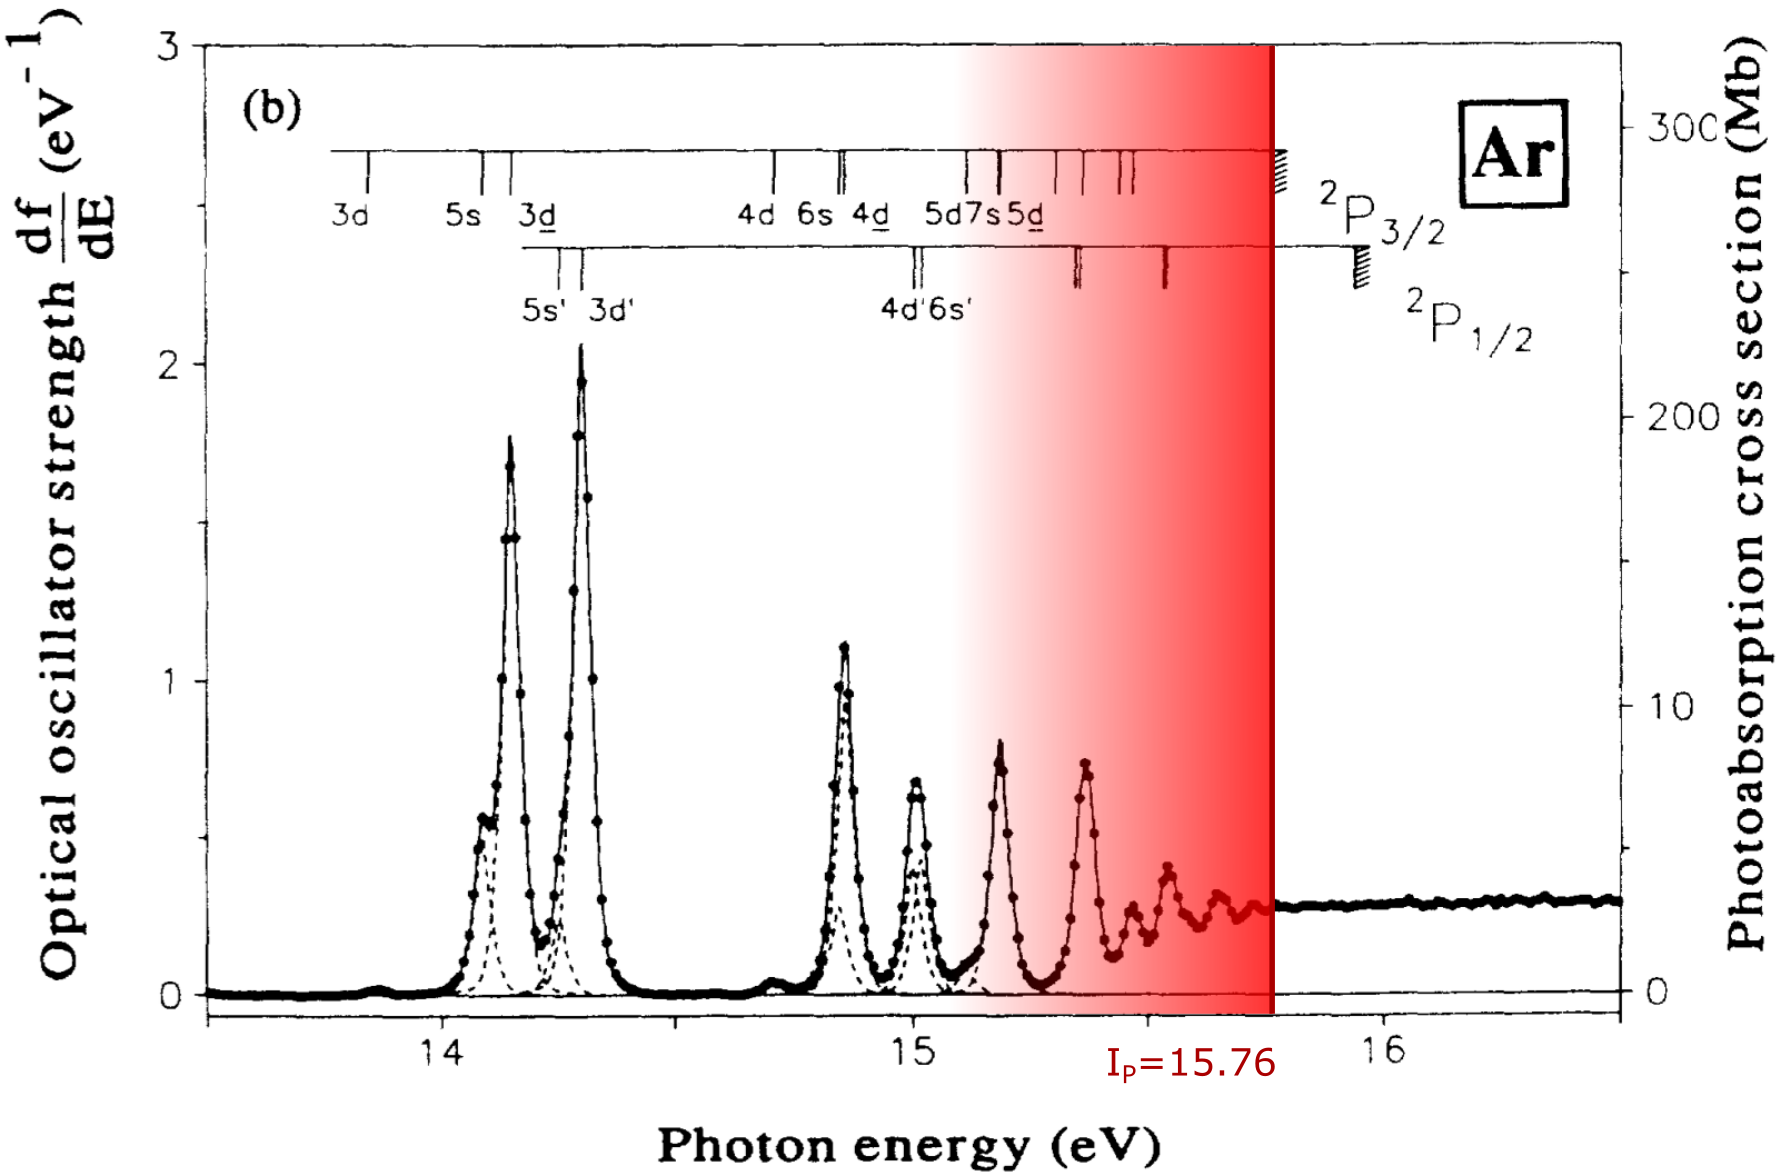
\includegraphics[width=0.9\columnwidth]{Figures/ResonantArgon/argon_spectrum.png}%
\caption{Section efficace de photoabsorption de l'argon dans la gamme 13.5-16.5 eV. Les lignes pointillées correspondent aux pics déconvolués. Tiré de \mycite{ChanPRA1992}.}
\label{fig:ArIp}%
\end{figure}

Nous allons voir que cette structure bien particulière donne lieu à plusieurs phénomènes intéressants. L'argon est un système de choix car son potentiel d'ionisation ($I_p = \SI{15.76}{eV}$) est très proche de l'énergie de 10 photons d'un laser Ti:Sa ($10\times 1.55 = 15.5$ eV). L'étude de la GHOE au voisinage du potentiel d'ionisation a été réalisée expérimentalement par \mycite{ChiniNP2014}, qui observèrent une émission à la fois en dessous et au dessus du seuil. Cette émission semble avoir des caractéristiques inhabituelles par rapport à la GHOE classique. En particulier, les auteurs remarquent une augmentation du signal avec la pression sans observer de phénomène de saturation, mais n'expliquent pas le mécanisme sous-jacent. Ensuite, \mycite{XiongPRL2014} et surtout \mycite{CampPRA2015} expliquent ce mécanisme en détail et montrent qu'il est lié à la présence des états de Rydberg de la figure \ref{fig:ArIp}. Deux effets distincts interviennent dans la génération.

Le premier est un mécanisme de GHOE résonante ayant lieu pendant l'ionisation de l'atome. Pendant la durée du pulse, tous les niveaux énergétiques de l'atome sont décalés par effet Stark. Pour les états de Rydberg de la figure \ref{fig:ArIp}, ce décalage vaut environ $U_p$, l'énergie pondéromotrice \mycite{GaardePRA2001,FiguieraPRA2002}. Ainsi, l'énergie d'un de ces niveaux peut devenir égale à l'énergie de $n$ photons infrarouges (dans notre cas, $n=10$). On a alors une résonance multi-photonique, qui augmente drastiquement l'intensité de la $n$-ième harmonique. La condition de résonance s'écrit : $n\hbar\omega = |E_R-E_0|+U_p$, où $E_R$ et $E_0$ sont respectivement les énergies de l'état fondamental et de l'état de Rydberg. Ce phénomène était déjà connu en ionisation au-dessus du seuil (ATI pour \textit{Above Threshold Ionization}) avec des impulsions courtes \mycite{FreemanPRL1987,AgostiniPRL1989}. On remarquera que pour l'argon, l'ordre harmonique résonant est le 10ème, qui n'est pas généré dans les conditions habituelles. Pour observer cet effet, on utilisera donc soit des impulsions infrarouges très courtes, soit on choisira une autre longueur d'onde de génération. Dans la suite, nous utiliserons une longueur d'onde de 400 nm, pour laquelle on a une résonance à 5 photons au seuil de l'argon.

Le second effet ne correspond pas à la GHOE, mais produit quand même un rayonnement ultraviolet dans cette région. Dans ce mécanisme, le faisceau infrarouge crée une superposition d'état cohérente entre l'état fondamental d'énergie $E_0$ et quelques états de Rydberg d'énergie $E_R$, via une transition multiphotonique. Le dipôle ainsi créé émet une radiation d'énergie $E_R-E_0$ pendant une durée correspond à la durée de vie de l'état de Rydberg, c'est-à-dire bien plus longtemps que l'émission harmonique. Ce rayonnement a donc une structure spectrale très fine. Ce processus s'appelle \textit{Free Induction Decay} ultraviolet (xFID) \mycite{BengtssonLarsenEtAl2015}, et était déjà connu en Résonance Magnétique Nucléaire \mycite{BlockPR1946} et dans l'infrarouge \mycite{BrewerPRA1972}. 

L'influence de ces deux effets a été étudiée expérimentalement en détail au CELIA Bordeaux par \mycite{beaulieuArXiv2016}. Des expériences réalisées à 800 nm ont permis d'observer les rayonnements issus de chacun de ces deux effets et d'étudier leurs propriétés de cohérence temporelle. Un spectre typique obtenu avec une impulsion de 7 fs est présenté sur la figure \ref{fig:xFID}. Les auteurs démontrent également la possibilité d'avoir ionisation à partir d'un état de Rydberg excité et recombinaison sur l'état fondamental, ce qui donne l'émission pointée par la ligne violette sur la figure \ref{fig:xFID}. 

\begin{figure}[!ht]
\centering
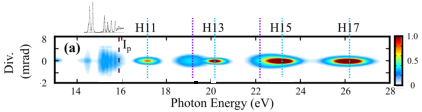
\includegraphics[width=1.1\columnwidth]{Figures/ResonantArgon/xFID.pdf}%
\caption{Spectre obtenu dans l'argon avec une impulsion de 7 fs à 800 nm. L'intensité est de $\SI{5.2e13}{W/cm^2}$. On observe le rayonnement xFID en dessous du seuil d'ionisation, que l'on compare avec le spectre d'absorption tiré de la figure \ref{fig:ArIp}. Ensuite, on observe les harmoniques non résonantes (lignes verticales bleues) ainsi que celles provenant d'états de Rydberg excités (lignes verticales violettes). Tiré de \mycite{beaulieuArXiv2016}.}
\label{fig:xFID}
\end{figure}



\subsection{Ellipticité du rayonnement près du seuil de l'argon}
\label{sec:resonant_argon_exp}
Pour avoir une résonance multiphonique au seuil de l'argon, nous choisissons de travailler à 400 nm. L'utilisation de cette longueur d'onde a deux autres avantages : (1) La GHOE est plus efficace, l'efficacité évolue en effet en $\lambda^{\simeq-6}$ \mycite{ShinerPRL2009}. (2) La largeur spectrale entre chaque harmonique est doublée et l'énergie de coupure diminue, on aura donc très peu d'harmoniques. Comme on le verra, ceci est très favorable dans les expériences de dichroïsme circulaire présentées plus loin. 

Ces expériences et toutes celles qui vont suivre ont été réalisées sur le système Aurore du CELIA Bordeaux, qui délivre des impulsions de 8mJ, 25 fs à environ 800 nm et à un taux de répétition de 1 kHz. Ce faisceau est ensuite doublé en fréquence par un BBO de type 1 et de $\SI{200}{\micro\meter}$ d'épaisseur. On mesure qu'à partir de 4 mJ du fondamental, on obtient 1 mJ à 404 nm. Le 800 nm restant est filtré à l'aide de miroir dichroïques, tandis que le 400 nm est focalisé par une lentille mince de Si$\text{O}_\text{2}$ de 50 cm de focale. Le reste du dispositif est similaire à celui présenté sur la figure \ref{Fig:ExpG} : des harmoniques sont générées dans un jet de gaz continu (ouverture de $\SI{300}{\micro\meter}$) puis imagées par un réseau de diffraction couplé à une galette de micro-canaux. 

Dans ce dispositif de GHOE assez typique, nous souhaitons rajouter une mesure de l'état de polarisation du rayonnement. Nous choisissons de mesurer des \textit{loi de Malus}. Habituellement, ces lois sont obtenues en mesurant l'intensité transmise par un polariseur parfait en fonction de l'angle du polariseur $\theta_p$ par rapport au champ électrique. Si le champ électrique est polarisé linéairement, l'intensité sera totalement transmise lorsque le polariseur est orienté parallèlement à la direction de polarisation du champ, et non transmise s'il est orthogonal. A contrario, si le champ est circulaire, l'intensité transmise ne variera pas en fonction de $\theta_p$. De manière générale, on obtient un signal oscillant de la forme 
\[I(\theta_p) = \epsilon^2+(1-\epsilon^2)\cos^2(\eta-\theta_p),\]
où $\epsilon$ et $\eta$ ont été définis dans la partie \ref{sec:polardef}. Remarquons que ce type de mesure est insensible à la partie non polarisée de la lumière, dont la contribution ne dépend pas de $\theta_p$. Ainsi, la valeur d'$\epsilon$ mesurée ici est encore une fois uniquement une borne supérieure, $\epsilon^{max}$. On voit donc que seulement pour une onde totalement polarisée, la mesure d'une loi de Malus donne accès à tous les paramètres de Stokes, définis plus haut. 

Il reste donc à réaliser un polariseur pour le rayonnement harmonique. Nous avons déjà mentionné que les surfaces métalliques présentaient des réflexions $R_s$ et $R_p$ différentes selon chaque dimension transverse (voir section \ref{sec:metalsurface}). Ainsi, en utilisant plusieurs de ces surfaces à la suite, on peut quasiment filtrer la composante $s$ ou $p$. Nous choisissons d'utiliser trois miroirs avec revêtement en or placés à 75\degres-60\degres-75\degres, ce qui donne un rapport total $R_s/R_p$ valant 5 à 20 pour la gamme spectrale étudiée. Enfin, plutôt que de motoriser et de faire tourner ce polariseur sous vide, on préfère tourner l'orientation du champ de génération et garder le polariseur fixe, ce qui est équivalent. Ce polariseur imparfait doit être pris en compte dans l'analyse de la loi de Malus (voir \mycite{AntoinePRA1997} ainsi que \mycite{gruson}), mais n'empêche pas de mesurer les paramètres recherchés, comme l'illustre la figure \ref{fig:malus} pour l'harmonique 5. Pour plus de détail sur ce dispositif de polarimétrie harmonique on se reportera à la thèse d'Amélie Ferré \mycite{ferre}.

\begin{figure}[!ht]
\centering
\def\svgwidth{0.7\columnwidth}
\import{Figures/ResonantArgon/}{malus.pdf_tex}
\caption{Lois de Malus pour l'harmonique 5 du faisceau à 404 nm. On mesure l'intensité transmise par le polariseur XUV en fonction de la direction de polarisation du champ de génération, lorsqu'il est polarisé linéairement (rouge) ou elliptiquement (vert). On voit que le champ harmonique est maximal en $\theta_p = \eta$, ce qui donne la direction de son ellipse de polarisation. Par ailleurs, on observe une diminution du contraste des oscillations avec $\epsilon_{IR}$, signe d'une ellipticité harmonique plus élevée. L'analyse des oscillations donne ici $\epsilon_q^{max} \simeq 0.6$ quand $\epsilon_{IR}=0.287$.}
\label{fig:malus}
\end{figure}

La figure \ref{fig:resonant_argon_exp} présente les résultats obtenus lorsque le laser de génération porte une ellipticité $\epsilon_{IR} = 0.4$. On observe les harmoniques 5, 7 et 9 du fondamental à 404 nm. Les harmoniques 7 et 9 présentent un profil gaussien spectralement, tandis que l'harmonique 5 est structurée. Cette structure est due au xFID, effet présenté plus haut. Le rayonnement xFID est superposé à l'émission harmonique, qui est résonante due à la résonance à 5 photons.  On mesure ensuite l'ellipticité en fonction de l'énergie de photon. On voit que l'ellipticité apparente des harmoniques non résonantes est de l'ordre de $\epsilon_{IR}$, tandis que celle de l'harmonique résonante est presque doublée (valeur maximale de 0.77).  

\begin{figure}[!ht]
\centering
\def\svgwidth{1\columnwidth}
\import{Figures/ResonantArgon/}{exp_result.pdf_tex}
\caption{Mesure d'ellipticité dans l'argon près du seuil d'ionisation. Le laser à 404 nm a une ellipticité de $\epsilon_{IR}=0.4$. Sur l'échelle de gauche (bleue), intensité en fonction de l'énergie de photon. On observe trois harmoniques, desquelles on mesure l'ellipticité apparente. On obtient les courbes rouges, échelle de droite.}
\label{fig:resonant_argon_exp}
\end{figure}

Pour confirmer que cette forte ellipticité est due à la présence de résonances, Bernard Pons et Baptiste Fabre, du CELIA Bordeaux, ont réalisé une étude théorique du problème. On résout l'équation de Schrödinger dépendante du temps (TDSE, \textit{Time-Dependant Schrödinger Equation}) à deux dimensions, en utilisant un potentiel de Coulomb de "cœur mou", qui reproduit la présence du potentiel d'ionisation et des états sous-jacents. La figure \ref{fig:resonant_argon_th_bound} illustre ce potentiel ainsi que le spectre harmonique obtenu. On observe des structures spectrales similaires à l'expérience, à la fois dans l'intensité et dans l'ellipticité de l'harmonique 5. L'ellipticité est en particulier très modulée, mais ne prend pas des valeurs aussi élevées que celles mesurées. Au contraire, elle devient même négative à 14 eV. Les calculs ont été répétés et ont permis d'observer qu'une très légère modification du potentiel atomique donnaient lieu à de très fortes modifications de l'ellipticité. On s'attend donc à n'avoir qu'un accord qualitatif.

\begin{figure}[!ht]
\centering
\def\svgwidth{1\columnwidth}
\import{Figures/ResonantArgon/}{th_result_bound.pdf_tex}
\caption{Résultat théorique en utilisant un potentiel de Coulomb de cœur mou. En haut, on représente le profil de ce potentiel, qui peut être ajusté pour obtenir la bonne valeur d'$\text{I}_{\text{p}}$. En bas, mêmes grandeurs que celles mesurées expérimentalement sur la figure \ref{fig:resonant_argon_exp}.}
\label{fig:resonant_argon_th_bound}
\end{figure}

En conclusion, nous voyons que la présence de résonances sous le seuil induit une modulation de l'ellipticité. Nous mesurons de plus qu'elle augmente très fortement. On obtient donc un rayonnement aux propriétés intéressantes sans véritable perte de signal : une mesure par une photodiode calibrée montre que l'harmonique 5 contient $\num{7e6}$ photons par impulsion. De plus, le caractère résonant de l'harmonique 5 fait qu'elle ne subit pas d'effet de réabsorption \mycite{ChiniNP2014}. Son flux peut donc être facilement augmenté par une pression de génération plus élevée.  Toutefois, cette méthode est restreinte à des énergies de photons relativement basses, correspondant au seuil d'ionisation du gaz utilisé. Les gaz habituellement utilisés pour avoir un flux important sont l'argon, $\text{I}_{\text{p}}=15.76$ eV, le krypton, $\text{I}_{\text{p}}=14$ eV, ou le xénon, $\text{I}_{\text{p}}=12.13$ eV. Il serait donc intéressant de généraliser notre approche à d'autres résonances d'énergie plus élevée. Dans la section suivante, nous étudions le cas de résonances dans le continuum.

\section{Génération autour d'une résonance dans le continuum}
Ces résonances se manifestent de la même façon que celles présentées plus haut : une augmentation de la section efficace de photoionisation. Nous nous intéressons au cas des \textit{résonances de forme} \mycite{Dehmer1972}, couramment observées dans le spectre de petites molécules. Bien qu'elles aient été observées assez tôt, leur interprétation et leur définition fait régulièrement débat, comme en témoigne l'article de \mycite{Piancastelli1999}, intitulé "\textit{The neverending story of shape resonances}" . Une interprétation courante est la suivante. Ces résonances sont dues à une barrière présente dans le potentiel moléculaire. Cette barrière est la résultante de forces attractives (e.g. coulombienne) et répulsives (effets d'écrantage, force centrifuge). Quand un photoélectron possède l'énergie correspond à cette barrière, il se retrouve dans un état métastable \mycite{simons1984roles}, piégé dans la barrière de potentiel, dont il finit par s'échapper par effet tunnel. La figure \ref{fig:shaperesonance} illustre ce principe : à l'énergie résonante, la fonction d'onde électronique est localisée sur le puit central et temporairement piégée.

\begin{figure}[!ht]
\centering
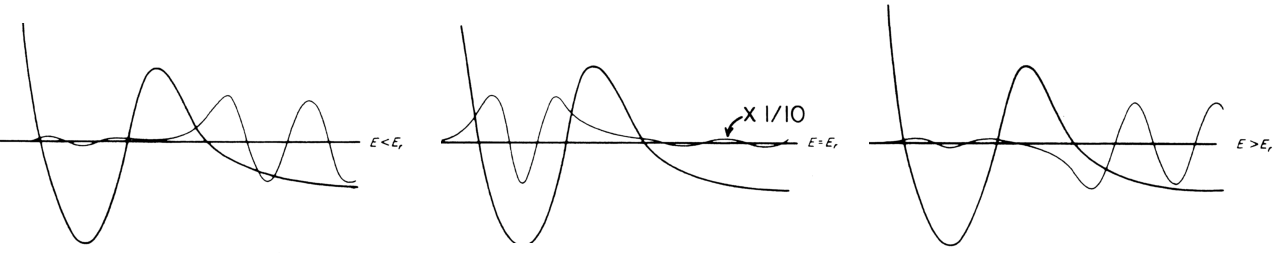
\includegraphics[width=1\columnwidth]{Figures/ResonantArgon/shape_resonance.pdf}%
\caption{Principe d'une résonance de forme. De gauche à droite, $E<E_r$, $E=E_r$ et $E>E_r$, où $E$ et $E_r$ sont les énergies du photoélectron et de la résonance. Tiré de \mycite{Piancastelli1999}.}
\label{fig:shaperesonance}
\end{figure}

De par sa nature, cette barrière de potentiel se situe relativement proche de la molécule. L'électron est ainsi spatialement localisé, ce qui augmente la densité électronique et produit en général un signal de photoionisation intense. Un autre intérêt de ces résonances et que la présence d'une barrière est liée à la forme de la molécule, d'où son nom. Ainsi, de nombreux travaux ont essayé de relier l'énergie des résonances de forme aux longueurs de liaisons de molécules adsorbées, méthodes astucieusement baptisées "\textit{Bond length with a ruler}" \mycite{StohrPRL1984}.

Nous étudions ici cet effet en ajoutant une barrière au potentiel de la figure \ref{fig:resonant_argon_th_bound} pour induire une résonance de forme vers l'énergie de l'harmonique 7. Ce potentiel ne correspond pas forcément à un système physique, mais nous permet de démontrer l'effet de la résonance du continuum. Le spectre obtenu est présenté sur la figure \ref{fig:resonant_argon_th_continuum}. On y voit le potentiel choisi, ainsi que la position de la résonance de forme. En orange, on représente une seconde résonance assez large du continuum, apparue après la modification du potentiel.

\begin{figure}[!ht]
\centering
\def\svgwidth{1\columnwidth}
\import{Figures/ResonantArgon/}{th_result_continuum.pdf_tex}
\caption{Résultat théorique en utilisant un potentiel de Coulomb de cœur mou auquel on ajoute une barrière. Le potentiel est représenté en haut de la figure. La ligne turquoise indique la position de la résonance de forme, tandis que la zone orange est une résonance large dans le continuum également apparue après modification du potentiel. En bas, mêmes grandeurs que celles mesurées expérimentalement sur la figure \ref{fig:resonant_argon_exp}.}
\label{fig:resonant_argon_th_continuum}
\end{figure}

Nous voyons donc que l'ellipticité de l'harmonique 7 et 9 sont significativement augmentés par la présence des deux résonances. La relation entre résonance et haute ellipticité est donc générale, ce qui permet de générer un rayonnement elliptique dans de nombreuses gammes énergétiques. Comment maintenant comprendre physiquement l'augmentation de cette ellipticité ? \mycite{StrelkovPRL2010} décrit théoriquement la GHOE près d'une résonance d'autoionisation, qui apparaît également lorsque le potentiel présente une barrière. Il montre que le modèle à trois étape habituel doit être modifié : au moment de la recombinaison, l'électron est piégé par la barrière de potentiel, le système se retrouve donc dans un état résonant du même type que celui de la figure \ref{fig:shaperesonance} avant de finalement se relaxer vers l'état fondamental en émettant un rayonnement XUV. Ce processus explique l'augmentation du signal harmonique près de la résonance par une forte section efficace de diffusion inélastique (qui contrôle le peuplement de l'état résonant) ainsi qu'une forte force d'oscillateur pour la transition entre l'état résonant et l'état fondamental.
Cette interprétation est tout à fait analogue à celle d'une résonance de forme en photoionisation donnée plus haut, ce qui illustre bien le caractère conjugué de ces deux effets.

Pour vérifier que l'ellipticité est bien créée par cette étape de piégeage, Bernard Pons et Baptiste Fabre ont effectué des calculs TDSE au moment de la recombinaison. On s'intéresse au paquet d'onde électronique d'abord ionisé, qui se propage puis recombine sur l'état fondamental. Le potentiel est le même que celui présenté sur la figure \ref{fig:resonant_argon_th_continuum}. Ce paquet d'onde $\Psi(\bm{r},t)$ se décompose sur une base d'états propres de l'hamiltonien du système (voir Supplementary Information de \mycite{FerreNP2015} pour plus de détails) :
\[ \Psi(\bm{r},t)=\sum_{E_n>0,l} a_{E_n,l}^{(o,e)}(t)\phi_{E_n,l}^{(o,e)}(\bm{r})e^{-(\rmi E_n t)},\]
où $\phi_{E_n,l}^{(o,e)}$ est l'état propre d'énergie $E_n$, positive puisqu'on cherche les électrons dans le continuum, de moment angulaire $l$, et $a_{E_n,l}^{(o,e)}$ est l'amplitude. $(o,e)$ correspondent à la symétrie de l'état par rapport à l'axe $\bm{e_x}$. Si on considère la recombinaison sur un état fondamental de symétrie $s$, seulement $\phi_{E_n,1}^{e}$ et $\phi_{E_n,1}^{o}$ contribuent. Ils correspondent respectivement à l'état propre parallèle $p_x$ et perpendiculaire $p_y$. La probabilité de trouver l'électron dans un de ces états est $P_{x,y}(E_n,t) = |a_{E_n,l}^{(o,e)}(t)|^2$. On choisit $E_n$ proche de l'énergie de résonance et on considère des instants proches de l'instant de recombinaison correspondant à l'harmonique 7. Les probabilités $P_x$ et $P_y$ sont représentées sur la figure \ref{fig:resonant_proba}.

\begin{figure}[!ht]
\centering
\def\svgwidth{1\columnwidth}
\import{Figures/ResonantArgon/}{electron_dynamics_resonance.pdf_tex}
\caption{\'{E}volution temporelle des probabilités $P_x$ (tirets bleus) et $P_y$ (traits pleins rouges) du paquet d'onde électronique arrivant sur un système présentant une résonance de forme. Le champ électrique a un cycle optique à 400 nm, une intensité pic de $\SI{10e14}{W/cm^2}$ et une ellipticité de 0.3.}
\label{fig:resonant_proba}
\end{figure}

Nous observons que la probabilité perpendiculaire $P_y$ augmente graduellement, jusqu'à dépasser $P_x$. Ceci signifie que la résonance de forme modifie géométriquement le paquet d'onde électrique alors qu'il s'approche de l'atome. Cette augmentation de $P_y$ se manifeste dans la GHOE par une augmentation de la composante perpendiculaire du champ émis et donc de son l'ellipticité.

\section{Application à la molécule de \sf6}
\label{sec:sf6ghoe}
Nous appliquons maintenant expérimentalement ce résultat. L'équipe du CELIA Bordeaux a étudié en détail la génération d'harmoniques dans un gaz de molécules de \sf6 (hexafluorure de soufre). Cette molécule a une structure octaédrique avec l'atome de soufre en son centre. Le panneau du haut de la figure \ref{fig:sf6_cross_section} montre la section efficace de photoionisation de \sf6. Le canal noté C correspond à une résonance d'autoionisation \mycite{fano1968}, tandis que le canal noté A est une résonance de forme. Un calcul numérique donne la contribution de ces canaux à la GHOE (panneau du bas), qui permet de voir que la génération autour des ordres 15 à 19 est dominée par ces deux canaux. On s'attend donc à avoir un transfert efficace d'ellipticité dans cette région spectrale.

\begin{figure}[!ht]
\centering
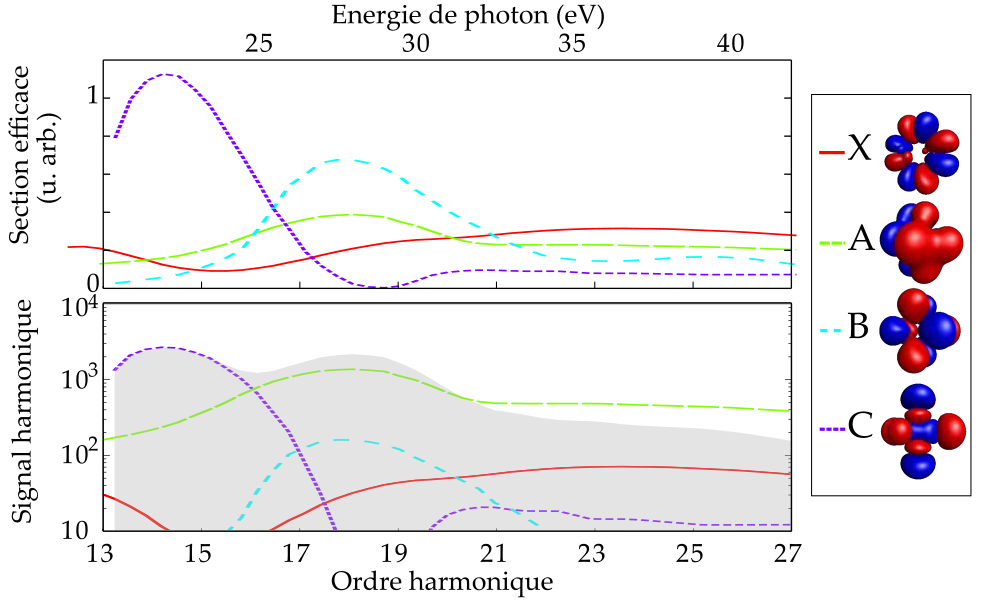
\includegraphics[width=.8\columnwidth]{Figures/SF6/sf6_cross_section.png}%
\caption{(Haut) Section efficace de photoionisation XUV de différents canaux d'ionisation. Extrait de \mycite{Yang98}. (Bas) Intensités des harmoniques générées par chaque canal, obtenues numériquement. La zone grisée est la superposition cohérente de tous les canaux d'ionisation. La longueur d'onde du champ de génération est 800 nm. (Droite) Orbitales moléculaires correspondant à chaque canal. Tiré de \mycite{FerreNC2015}.}
\label{fig:sf6_cross_section}
\end{figure}

Nous avons mesuré l'ellipticité apparente du rayonnement dans cette gamme spectrale en utilisant le polariseur décrit plus haut. Les résultats sont présentés sur la figure \ref{fig:sf6_ell}. Dans un premier temps, on utilise un champ de génération à 800 nm. On observe de très hautes valeurs d'ellipticité pour les harmoniques résonantes, atteignant presque 0.8 pour l'harmonique 15 avec seulement une ellipticité de génération de 0.2. 

\begin{figure}[!ht]
\centering
\def\svgwidth{1\columnwidth}
\import{Figures/SF6/}{sf6_ellipticite.pdf_tex}
\caption{En haut, signal harmonique produit dans \sf6 en variant l'ellipticité de génération $\epsilon_0$. En marron à jaune, impulsions de 800 nm, $\SI{1.3e14}{W/cm^2}$. En bleu foncé à clair, impulsions de 400 nm, $\SI{1.0e14}{W/cm^2}$. En bas, ellipticité apparente du rayonnement harmonique. L'erreur sur la mesure, déterminée en répétant les mesures, est de $\pm0.03$.}
\label{fig:sf6_ell}
\end{figure}

Pour les mêmes raisons qu'expliqué auparavant, il est avantageux d'utiliser un laser de génération à 400 nm. L'expérience montre que l'on garde une ellipticité très satisfaisante : les harmoniques 5 et 7 portent respectivement une ellipticité de $\simeq 0.75$ et $\simeq 0.5$ avec $\epsilon_0=0.45$. On dispose ainsi d'une source aux propriétés remarquables, le flux étant amélioré par la génération à 400 nm. Une mesure par une photodiode calibrée montre que l'harmonique 5 contient $\num{7e6}$ photons par impulsion quand $\epsilon_0=0.3$, c'est-à-dire $\num{2e9}$ photons par seconde. Cette valeur peut être encore augmentée en utilisant par exemple des impulsions plus énergétiques et une longueur focale plus élevée.

En conclusion, nous avons construit une source de rayonnement ultraviolet ultra-bref polarisé circulairement. Chaque harmonique considérée séparément a en effet une durée de l'ordre de la durée de l'impulsion de génération, c'est-à-dire $\simeq 20$ femtosecondes, ce qui en fait une alternative particulièrement intéressante aux sources synchrotrons malgré son flux moindre. Comparé aux lasers à électron libre, eux aussi capables de produire des polarisation circulaires \mycite{AllariaPRX2014}, le flux est bien sûr bien moindre, mais le taux de répétition et la résolution temporelle fournis par la GHOE sont très avantageux pour des mesures de spectroscopie moléculaire. Dans la suite nous démontrerons ce point en effectuant des expériences de photoionisation sur des molécules chirales. 
%
\chapter{Polarisation circulaire et chiralité}
\section{Définitions de la chiralité}
\subsection{Molécules chirales}
Le concept de polarisation de la lumière est historiquement lié à celui de la \textit{chiralité}. En 1808, Malus observa que la lumière réfléchie par une substance diaphane possédait une polarisation (mot qu'il introduisit en 1810). Cette polarisation était mise en évidence par une transmission à travers un cristal de calcite. Cette propriété fut observée par Arago dans des cristaux de quartz, avant d'être étudiée par Biot qui en 1812 montra que différents types de quartz tournaient la direction de polarisation soit à droite soit à gauche, propriété appelée \textit{activité optique}. Il mesura le même effet dans des substances organiques telles que des molécules de camphre. En 1848, Pasteur relia cette propriété optique à la géométrie du cristal ou de la molécule considérée. Il émit l'idée que certaines molécules existaient sous des formes géométriques dissymétriques tout en ayant les mêmes propriétés chimiques. Le mot de \textit{chiralité} fut introduit en 1893 par Lord Kelvin durant la deuxième "Robert Boyle Lecture" à l'université d'Oxford \mycite{kelvin1894} :
\begin{quotation}
I call any geometrical figure, or group of points, 'chiral', and say that it has chirality if its image in a plane mirror, ideally realized, cannot be brought to coincide with itself.
\end{quotation}
Le terme de chiralité dérive du mot grec sigifiant "main", un exemple d'objet chiral (voir figure \ref{fig:chirality}). Les deux formes possèdent un pouvoir rotatoire opposé et sont nommées \textit{énantiomères} (formes opposées en grec). On peut les nommer selon le signe de la rotation qu'ils imposent à la lumière : on parle alors de molécule dextrogyre (D ou +) ou lévogire (L ou -). Cependant, une même molécule peut imposer une rotation gauche ou droite selon la longueur d'onde de la lumière utilisée. On utilise donc également la configuration absolue de la molécule, définie à partir de sa structure tri-dimensionelle. On note alors les énantiomère R (rectus) et S (sinister). La configuration absolue d'une molécule est habituellement mesurée par diffraction X \mycite{Bijvoet1951}, par explosion coulombienne \mycite{pitzer2013} ou encore par spectroscopie micro-onde \mycite{patterson2013}.

\begin{figure}[!ht]
\centering
\includegraphics[width=.5\columnwidth]{Figures/Chirality/chirality_with_hands.pdf}%
\caption{Une molécule "chirale" n'est pas superposable à son image dans un miroir. De même que les mains gauches et droites ont un pouce et des doigts dans le même ordre, les molécules chirales ont les mêmes atomes dans le même ordre mais ne sont pas images l'une de l'autre dans un miroir.}
\label{fig:chirality}
\end{figure}

\subsection{La chiralité de la lumière}
Deux énantiomères ont les mêmes propriétés chimiques. Cependant, elles interagiront différemment avec un objet lui-même chiral. Par exemple, la plupart des récepteurs biologiques sont chiraux et réagiront très différemment à une protéine R ou S. Le contrôle et la mesure des propriétés chirales sont donc centraux dans l'industrie alimentaire, pharmaceutique et cosmétique. 

Les expériences mentionnées montrent que la lumière permet de caractériser une molécule chirale, ce qui implique que la lumière elle-même doit être un objet chiral. La définition donnée plus haut est insuffisante, car comme noté par Lord Kelvin dans ses \textit{Baltimore Lecture}, elle ne permet pas de distinguer les effets due à la chiralité de ceux dues à d'autres types de dissymétries telles que l'effet Faraday. \mycite{Barron1986} donne une définition généralisable à la chiralité de particules élémentaires telles qu'un photon :

\begin{quotation}
True chirality is exhibited by systems that exist in two distinct enantiomeric (enantiomorphic) states that are interconverted by space inversion, but not by time reversal combined with any proper spatial rotation.
\end{quotation}

Cette définition permet de distinguer la "vraie" chiralité de la fausse, c'est-à-dire une chiralité indépendante du temps. Les opérations spatiales et temporelles décrites sont représentées sur la figure \ref{fig:truefalsechir}, où elles sont notées T (inversion du temps), P (inversion de l'espace), et $\text{R}_{\pi}$ (rotation, ici d'angle $\pi$). 

\begin{figure}[!ht]
\centering
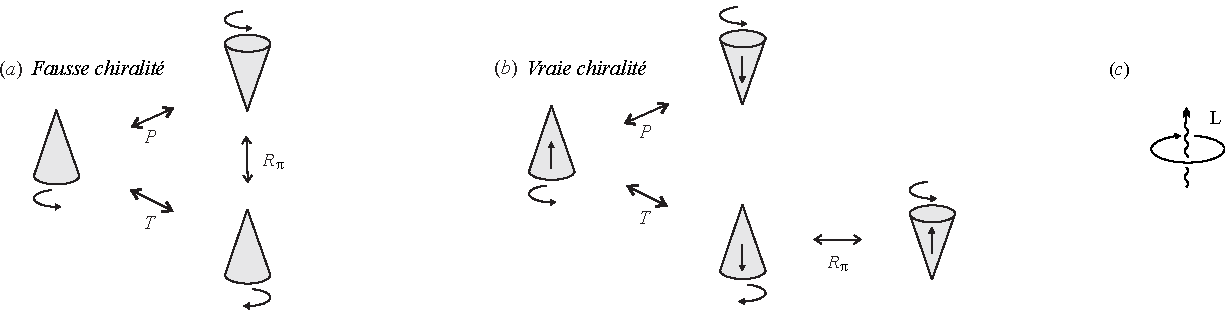
\includegraphics[width=.9\columnwidth]{Figures/Chirality/truefalsechir.pdf}%
\caption{Vraie et fausse chiralité. \textit{(a)} Cône en rotation immobile. P (inversion de l'espace) donne le même résultat que T (inversion du temps) suivi de $\text{R}_{\pi}$ (rotation d'angle $\pi$). \textit{(b)} Cône en rotation en translation. Il présente cette fois une vraie chiralité. \textit{(c)} Lumière polarisée circulairement : un photon est analogue au cône en translation. Tiré de \mycite{barron}.}
\label{fig:truefalsechir}
\end{figure}

Dans cette figure, on prend l'exemple d'un cône en rotation. Si le cône est immobile, P donne la même chose que T suivi de $\text{R}_{\pi}$, il ne présente pas de vraie chiralité. Au contraire, s'il est en translation, il a une vraie chiralité. Le cas du photon est similaire, l'hélicité du photon pouvant être vue classiquement comme une rotation. Le photon ne peut de plus pas être immobile, la lumière polarisée circulairement est donc chirale selon cette définition. Pour des molécules chirales, on appelle mélange \textit{racémique} un mélange composé d'autant de chacun des deux énantiomères. Ceci est analogue à une lumière polarisée linéairement, constituée d'autant de photons polarisés circulairement droit que gauche. 

La lumière polarisée circulairement est donc un outil de choix pour sonder et caractériser les molécules chirales. De nombreuses interactions sont possibles, nous décrirons dans la section suivante celle nommée dichroïsme circulaire, avant de présenter le dichroïsme circulaire de photoélectron, que nous mesurerons avec la source décrite dans la partie \ref{CH:Circular_HHG}.

\section{Dichroïsme circulaire d'absorption}
Fresnel expliqua le phénomène d'activité optique par une différence de vitesse de propagation de la composante circulaire droite (notée D) et gauche (G) d'une onde polarisée linéairement. Le milieu présente donc un indice de réfraction pour chaque composante. Considèrons un champ polarisé linéairement tel que les vecteurs champs électriques RCP et LCP soient parallèles à $z = 0$. Après une propagation sur une distance $L$, les champs auront tourné de $\theta^{G}=2\pi\rmc L/(\lambda v^{G})$ et $\theta^{R}=-2\pi\rmc L/(\lambda v^{RCP})$. L'angle de rotation de la direction du champ s'écrit alors :
\begin{align*}
\chi = \frac{1}{2}(\theta^{G}+\theta^{D}) &= \frac{\pi\rmc L}{\lambda}\left(\frac{1}{v^{G}}-\frac{1}{v^{D}}\right)\\
&= \frac{\pi}{\lambda}\left(n^{G}-n^{D}\right).
\end{align*}

Mais si $n^{G}$ et $n^{D}$ sont différents, le milieu doit également absorber différemment chaque composante du champ. Cet effet a été mesuré pour la première fois par \mycite{Haidinger1847} puis étudié par \mycite{Cotton1895}, qui le nomma \textit{dichroïsme circulaire}. Cet effet est toujours couramment utilisé avec des longueurs d'ondes visibles ou infrarouges. Il est généralement préféré à la mesure de l'activité optique car il évolue plus rapidement avec la longueur d'onde, et permet donc de distinguer plus facilement différentes bandes spectrales. Le dichroïsme circulaire est ainsi utilisé pour la détermination de structures de protéines, de changements de structures induits par par exemple le pH ou le solvant, de repliements/dépliements de protéines, ou encore de liaison de ligands.

L'absorption correspond à une transition d'un état initial vers un état excité. Lorsque la lumière traverse un ensemble de molécule, son intensité est gouvernée par la loi de Beer-Lambert, c'est-à-dire une décroissance exponentielle en fonction de la longueur parcourue. On note $\alpha^{D}$ et $\alpha^{G}$ les coefficients d'absorption de chacune des composantes du champ. Le dichroïsme circulaire vaut :
\[\Delta \alpha = \alpha^{G}-\alpha^{D}.\]
En pratique, on préfère utiliser le ratio entre le dichroïsme circulaire et l'absorption habituelle, appelé facteur de dissymétrie \mycite{Kuhn1930} : 
\begin{equation}
g = \frac{\alpha^{G}-\alpha^{D}}{\frac{1}{2}(\alpha^{G}+\alpha^{D})}.
\label{eq:kuhn}
\end{equation}

Relions $\alpha$ aux propriétés de la molécule. Pour une longueur de propagation $\delta z$ dans le milieu infinitésimale, l'intensité absorbée par unité de surface $\delta I$ s'écrit :
\begin{align*}
\frac{\delta I}{I} = \alpha c \delta z,
\end{align*}
où $c$ est le nombre de molécule par mètre cube. On note $w$ l'énergie moyenne absorbée par molécule, on a donc $\delta I = c \delta z w$. On obtient alors :
\begin{align}
\alpha = \frac{\delta I}{Ic \delta z} = \frac{c \delta z w}{Ic \delta z} = \frac{w}{I}.
\label{eq:cd1}
\end{align}
Notons qu'un facteur de proportionnalité s'ajoute à cette expression si on choisit d'utiliser un coefficient d'absorption molaire.

Considérons maintenant la transition électronique $i\rightarrow f$. \`A cette transition est associé un élément de matrice de transition qu'on note $V_{if}$. La bande d'absorption a un profil spectral qui donne la probabilité de transition en fonction de la fréquence, qu'on note $\rho(\omega)$. \mycite{schellman1975} montre que ces quantités sont reliés à $w$ par la relation :
\begin{equation}
w(\omega) = \frac{\pi \omega |V_{if}|^2 \rho(\omega)}{2\hbar}.
\label{eq:cd2}
\end{equation}

Il faut donc déterminer $V_{if}$ pour obtenir $\alpha$. Commençons dans l'approximation dipolaire électrique. Dans ce cas, le champ électrique se couple avec le moment dipolaire de la molécule : $V_{if} = -\bm{\mu}_{if}\cdot \bm{E}$, où $\mu_{if}$ est le moment dipolaire (voir partie \ref{sec:multipolar}). \mycite{schellman1975} montre que si le champ est polarisé circulairement droite ou gauche, on a $(V_{if}^{D/G})^2 = (\bm{\mu}_{if})^2E^2_0/3$, où la division par 3 provient d'une moyenne sur les orientation possibles des moments dipolaires.
On utilise alors les équations \ref{eq:cd1} et \ref{eq:cd2} :
\begin{align*}
\alpha^{D/G}(\omega) &= \frac{w^{D/G}(\omega)}{I} = \frac{\pi \omega |V_{if}^{D/G}|^2 \rho(\omega)}{2\hbar I} 
= \frac{\pi \omega |\mu_{if}E_0|^2 \rho(\omega)}{6\hbar I} 
= \frac{\pi \omega |\mu_{if}|^2 \rho(\omega)E^2_0}{6\hbar I} \\
&= \frac{4\pi^2 \omega |\mu_{if}|^2 \rho(\omega)}{3\hbar n \rmc} 
\end{align*}
On obtient donc directement le dichroïsme circulaire : $\Delta\alpha = \alpha^G-\alpha^D = 0$. Dans l'approximation dipolaire, le dichroïsme circulaire est donc nul. \par Il faut considérer le terme suivant du développement multipolaire : 
\[V_{if} = -\bm{\mu}_{if}\cdot \bm{E} - \bm{m}_{if}\cdot \bm{B}.\] 
\mycite{schellman1975} réalise le calcul de $V_{if}$ pour une polarisation circulaire :
\begin{align*}
(V_{if}^{D/G})^2 &= \frac{(\bm{\mu}_{if})^2E^2_0}{3}+\frac{(\bm{m}_{if})^2B^2_0}{3} \mp \frac{2}{3}\text{Im}(\bm{\mu}_{if}\cdot\bm{m}_{if})E_0B_0 \\
&= \frac{8\pi I}{3 \rmc}\left[\frac{(\bm{\mu}_{if})^2}{n} +  n(\bm{m}_{if})^2 \mp 2 \text{Im}(\bm{\mu}_{if}\cdot\bm{m}_{if})\right]. 
\end{align*}
Chacun des trois terme a sa propre probabilité de transition, qu'on note $\rho(\omega)$, $\tau(\omega)$ et $\sigma(\omega)$. On obtient donc pour le coefficient d'atténuation :
\begin{equation*}
\alpha^{D/G}(\omega) = \frac{4\pi^2 \omega}{3\hbar \rmc}\left[\frac{\rho(\omega)(\bm{\mu}_{if})^2}{n} +  n\tau(\omega)(\bm{m}_{if})^2 \mp 2 \sigma(\omega)\text{Im}(\bm{\mu}_{if}\cdot\bm{m}_{if})\right] 
\end{equation*}

Les trois termes obtenus correspondent à l'absorption dipolaire électrique, l'absorption dipolaire magnétique, et le dichroïsme circulaire. En effet, on obtient :
\[ \Delta \alpha = \alpha^G-\alpha^D = \frac{16\pi^2 \omega\sigma(\omega)\text{Im}(\bm{\mu}_{if}\cdot\bm{m}_{if})}{3\hbar \rmc}. \]
Le fait que l'on ait besoin d'utiliser l'approximation dipolaire magnétique pour observer du dichroïsme circulaire signifie que cet effet sera faible en général. Ainsi, le facteur d'asymétrie $g$ (équation \ref{eq:kuhn}) a des valeurs typiques de $10^{-5}\text{-}10^{-3}$ \mycite{Levi1980}. Ceci impose de réaliser des mesures à densité élevée, c'est-à-dire en phase liquide ou sur des films minces. La mesure est alors parasitée par la contribution du solvant ou du substrat, empêchant la mesure du dichroïsme de la molécule libre.
\clearpage
\section{Dichroïsme circulaire de photoélectron (PECD)}
\label{sec:PECD}
On s'intéresse désormais à un autre type de dichroïsme, qui comme nous allons voir a des propriétés très différentes. Jusque ici, nous avons présenté des techniques chiroptiques (terme désignant l'étude de molécule chirales par la lumière) dans le domaine visible ou proche infrarouge. Le passage à des énergies de photon plus élevées donne accès à un phénomène supplémentaire : la photoionisation. Nous allons donc décrire l'émission d'un électron par une molécule chirale suite à l'absorption de lumière polarisée circulairement. 

On considère une impulsion lumineuse se propageant selon la direction $e_z$. On place une molécule chirale au centre d'un repère sphérique $(r,\theta,\phi)$, où $r$ est la position du photoélectron, $\theta$ est l'angle par rapport à l'axe $e_z$, comme représenté sur la figure \ref{fig:geomPECD}.

\begin{figure}[!ht]
\centering
\def\svgwidth{0.5\columnwidth}
\import{Figures/PECD/}{geomPECD.pdf_tex}
\caption{Géométrie de photoionisation.}
\label{fig:geomPECD}
\end{figure}

Dans le cas de molécules chirales d'orientation aléatoire et d'un champ parfaitement polarisé, le phénomène ne dépend pas de $\phi$. En 1976, \mycite{RitchiePRA1976} obtint l'expression de la distribution angulaire des photoélectrons éjectés et montra qu'elle prend la forme suivante :
\begin{equation}
I^p(r,\theta) = b_0^p(r) + b_1^p(r) P_1(\cos\theta) + b_2^p(r) P_2(\cos\theta)
\label{eq:angulardistrib}
\end{equation}
où les $b_i$ sont des fonctions du potentiel moléculaire, de l'énergie $h\nu$ et de la polarisation $p$ du photon incident ($p = 0$, polarisation linéaire, $p =\pm1$ polarisation circulaire gauche/droite). Les $P_i$ sont les polynômes de Legendre, qui valent $P_1(x) = x$ et $P_2(x) = (3x^2-1)/2$. Il est important de noter que contrairement à celui du dichroïsme circulaire, ce calcul a été réalisé dans l'approximation dipolaire électrique. Le calcul complet des $b_i$ permet d'obtenir les propriétés suivantes :
\begin{align}
b_0^1 &= b_0^{-1} \nonumber\\
b_1^0 &= 0\nonumber\\
b_1^1 &= -b_1^{-1}\nonumber\\
b_2^1 &= b_2^{-1}.
\label{eq:bi}
\end{align}
$b_0$ est couramment appelé PES (Photo Emission Spectrum), et correspond simplement à la section efficace de photoionisation de la molécule. $b_2$ est souvent noté $\beta$ et appelé paramètre d'anisotropie. Quant à $b_1$, on remarque qu'il fait apparaître un dichroïsme :
\begin{equation}
I^{1}(r,\theta)-I^{-1}(r,\theta) = (b_1^1(r)-b_1^{-1}(r))P_1(\cos\theta) = 2b_1^1(r)\cos\theta
\label{eq:pecddef}
\end{equation}
On obtient donc une asymétrie autour de $\theta = 90\degres$, c'est-à-dire avant-arrière par rapport à la direction de propagation de la lumière. Cet effet est appelé dichroïsme circulaire de photoélectron (PECD, \textit{PhotoElectron Circular Dichroism}), et $b_1$ est le \textit{paramètre dichroïque}. On note souvent $PECD = 2b_1$. L'équation \ref{eq:bi} montre directement que le PECD change de signe si on change l'hélicité de la lumière. De même, le signe change si on change d'énantiomère.

\mycite{PowisJPCA2000} obtint théoriquement des asymétries allant jusqu'à 40\% de la section efficace totale. Des démonstrations expérimentales n'ont pas tardé à arriver, profitant du développement de sources synchrotrons fournissant de la lumière XUV polarisée circulairement. \mycite{BoweringPRL2001} ont mesuré le PECD du bromocamphre en 2001, avant que \mycite{GarciaJCP2003} étudient le camphre et \mycite{TurchiniJACS2004} le methyloxirane. L'asymétrie la plus haute aujourd'hui mesurée est de 32\% \mycite{DalyJCP2011}. Ces valeurs élevées s'expliquent par le caractère purement dipolaire électrique du PECD et permettent de réaliser des études chiroptiques en phase gazeuse.
Par la suite, l'étude du PECD a montré son impressionnante sensibilité aux finesses du potentiel moléculaire. Tout d'abord, $b_1$ est différent selon l'orbitale ionisée, comme démontré dans le camphre par \mycite{NahonJCP2006}. Ensuite, le PECD peut varier drastiquement avec des substitutions chimiques, comme illustré sur la figure \ref{fig:substitution}, tirée de \mycite{Tia2014}. On y voit qu'en changeant un élément de la molécule, la section efficace et le paramètre $\beta$ ne changent presque pas, car l'orbitale ionisée est localisé sur l'atome d'oxygène. Cependant, le paramètre $b_1$ évolue drastiquement, permettant de différencier les quatres molécules. Un autre exemple est celui des conformères, qui sont des molécules de même formule mais dont les atomes ont tourné autour d'une liaison chimique. Le PECD est également capable de distinguer ces deux molécules \mycite{GarciaPCCP2008}. Pour finir, il a récemment été observé que le PECD était sensible aux modes de vibration, c'est-à-dire aux mouvements des noyaux \mycite{GarciaNC2013}.

\begin{figure}[!ht]
\centering
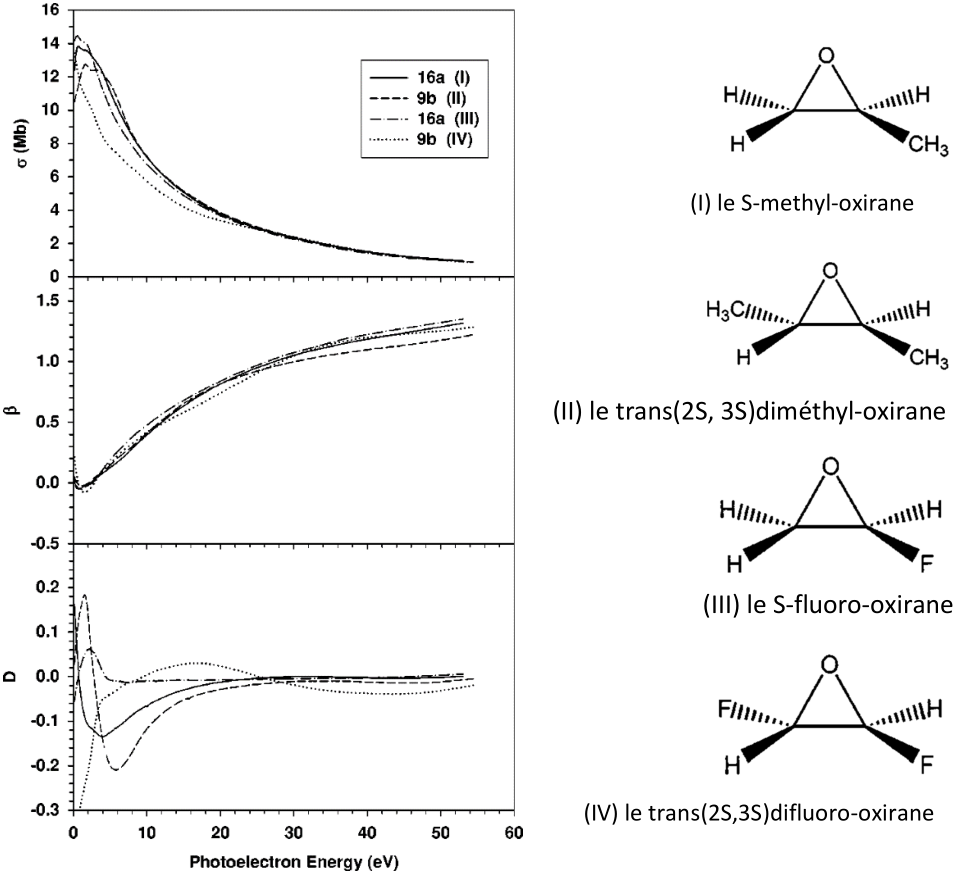
\includegraphics[width=.7\columnwidth]{Figures/PECD/substitution.png}%
\caption{Effet d'une substitution sur le PECD. Quatres molécules sont représentées à droite. \`A gauche, on voit leur section efficace de photoionisation $\sigma$, leur paramètre d'anisotropie $\beta$ et le paramètre dichroïque $b_1$, ici noté D. Tiré de \mycite{Tia2014}.}
\label{fig:substitution}
\end{figure}

Cette haute sensibilité au détails fins du potentiel moléculaire peut être expliquée dans un modèle où un électron diffuse sur la molécule après avoir été ionisé. On part d'un état initial où l'électron est lié, et on observe l'électron dans le continuum après qu'il ait diffusé sur le potentiel moléculaire. \mycite{DillDehmer1974} montrent que la fonction d'onde du photoélectron dans le continuum se décompose en différentes composantes de moment angulaire défini. Chacune de ces composante est déphasée différemment par le potentiel moléculaire. La phase de chaque composante $\ell$, que l'on note $\sigma_\ell$, est responsable d'interférences dans le continuum entre ondes partielles. Ainsi, une observable sera d'autant plus sensible au potentiel moléculaire qu'elle est sensible à des petites variations de $\sigma_\ell$. Le calcul de \mycite{RitchiePRA1976} donne les dépendances en $\sigma_\ell$ des $b_i$ :

\begin{itemize}
\renewcommand{\labelitemi}{$\bullet$}
\setlength\itemsep{1em}
\item $b_0$ ne dépend pas du tout de $\sigma_\ell$. La section efficace intégrée sur tout l'espace ne présente donc que peu d'information.
\item $b_2$ dépend de $\sigma_\ell$ pour une valeur de $\ell$ sur deux. Plus précisément, $b_2$ présente un terme $\cos(\sigma_\ell-\sigma_{\ell+2})$. $b_2$ fournit donc davantage d'information que la section efficace totale.
\item Le cas qui nous intéresse est celui de $b_1$, qui lui présente un terme $\sin(\sigma_\ell-\sigma_{\ell+1})$. Toutes les composantes $\ell$ influent donc sur sa valeur. De plus, on a une dépendance en sinus, qui varie significativement pour des petites valeurs de déphasage entre composantes $\ell$. Au contraire, le cosinus dans l'expression de $b_2$ est relativement plat au voisinnage de $\sigma_\ell-\sigma_{\ell+2} = 0$.
\end{itemize}

Nous avons jusque ici mentionné des études réalisées sur synchrotron. Ces travaux présentent une très bonne résolution spectrale, mais faute de source adaptée, aucune étude \textit{dynamique} du PECD n'a été réalisée. Nous allons utiliser la source présentée en partie \ref{CH:Circular_HHG} à cet effet.
%
\chapter{Mesures de PECD avec une source d'harmoniques d'ordre élevé}
\section{Dispositif expérimental}
\subsubsection{Source de lumière}
Nous utilisons la source décrite en partie \ref{CH:Circular_HHG}, dont nous rappelons brièvement les propriétés : le système laser Aurore délivre des impulsions à $\simeq$800 nm, qui sont doublées dans un cristal de BBO de type 1 de 200 $\si{\micro\metre}$. On dispose alors d'impulsions de 1 mJ à 404 nm à une fréquence de 1 kHz. Pour mesurer un PECD, il est pratique d'alterner successivement polarisations circulaires droite et gauche et de faire la différence entre elles, de sorte à éviter des effets de dérive lente. Pour ce faire, il faut alterner la polarisation du champ de génération à 404 nm. On utilise une lame demi-onde d'ordre 0 large bande placée avant une lame quart d'onde. L'orientation de la lame quart d'onde est fixe selon l'axe vertical. On peut ainsi tourner la lame demi-onde d'un angle $\pm\beta/2$ pour obtenir une ellipticité $\epsilon_0 = \pm \tan\beta$, tout en gardant l'axe de l'ellipse vertical après les lames d'onde. On choisit ici $\epsilon_0 = \pm 0.3$. La figure \ref{fig:waveplates} illustre le fonctionnement du dispositif. Le rayonnement est ensuite focalisé dans un jet de \sf6 par lentille de $\text{SiO}_2$ de 50 cm de focale. Les harmoniques générées sont alors polarisées elliptiquement et d'ellipticité de même signe que celui du fondamental. Les valeurs d'ellipticité apparentes ont été présentées plus haut (voir figure \ref{fig:sf6_ell}).

\begin{figure}[!ht]
\centering
\def\svgwidth{0.7\columnwidth}
\import{Figures/PECD/}{waveplates.pdf_tex}
\caption{Contrôle de l'état de polarisation du fondamental. De gauche à droite : état de polarisation avant les lames d'onde, état après une lame demi-onde d'angle $\pm\beta/2$, état après une lame quart d'onde orientée verticalement.}
\label{fig:waveplates}
\end{figure}

\subsubsection{Détection : spectromètre imageur de vecteur vitesse}
Le champ harmonique produit par les molécules de \sf6 est alors utilisé pour photoioniser un gaz de molécules chirales. Pour ne pas modifier l'état de polarisation du champ, on n'introduit aucune optique entre la source et la zone de détection. Seul un iris permet d'ajuster l'intensité envoyée dans le gaz de molécule. La mesure du PECD de ces molécules nécessite de connaître l'énergie et la direction d'émission des photoélectron créés lors de la photoionisation. Expérimentalement, ceci est réalisé à l'aide d'un spectromètre imageur de vecteur vitesse (VMI pour \textit{Velocity Map Imager}). 

Le fonctionnement de cet appareil est représenté sur la figure \ref{fig:vmi}. Le faisceau harmonique croise un jet moléculaire, dont le recouvrement définit la zone d'interaction. La photoionisation a lieu dans cette zone, et crée un nuage d'espèces chargées (ions et électrons). Autour de cette zone sont positionnées trois électrodes servant à collecter ces espèces chargées. Ces électrodes forment une \textit{lentille électrostatique} qui vient focaliser les espèces chargées sur un détecteur placé perpendiculairement à l'axe de propagation de la lumière, constitué de galettes de micro-canaux (MCP) et d'un écran de phosphore. L'électrode la plus éloignée du détecteur repousse les espèces et est donc appelée répulseur. L'électrode intermédiaire est appelée extracteur, tandis que la troisième est l'électrode de masse car son potentiel est nul. Le signe des potentiels permet de collecter les ions ou bien les électrons émis lors de l'interaction. 

\begin{figure}[!ht]
\centering
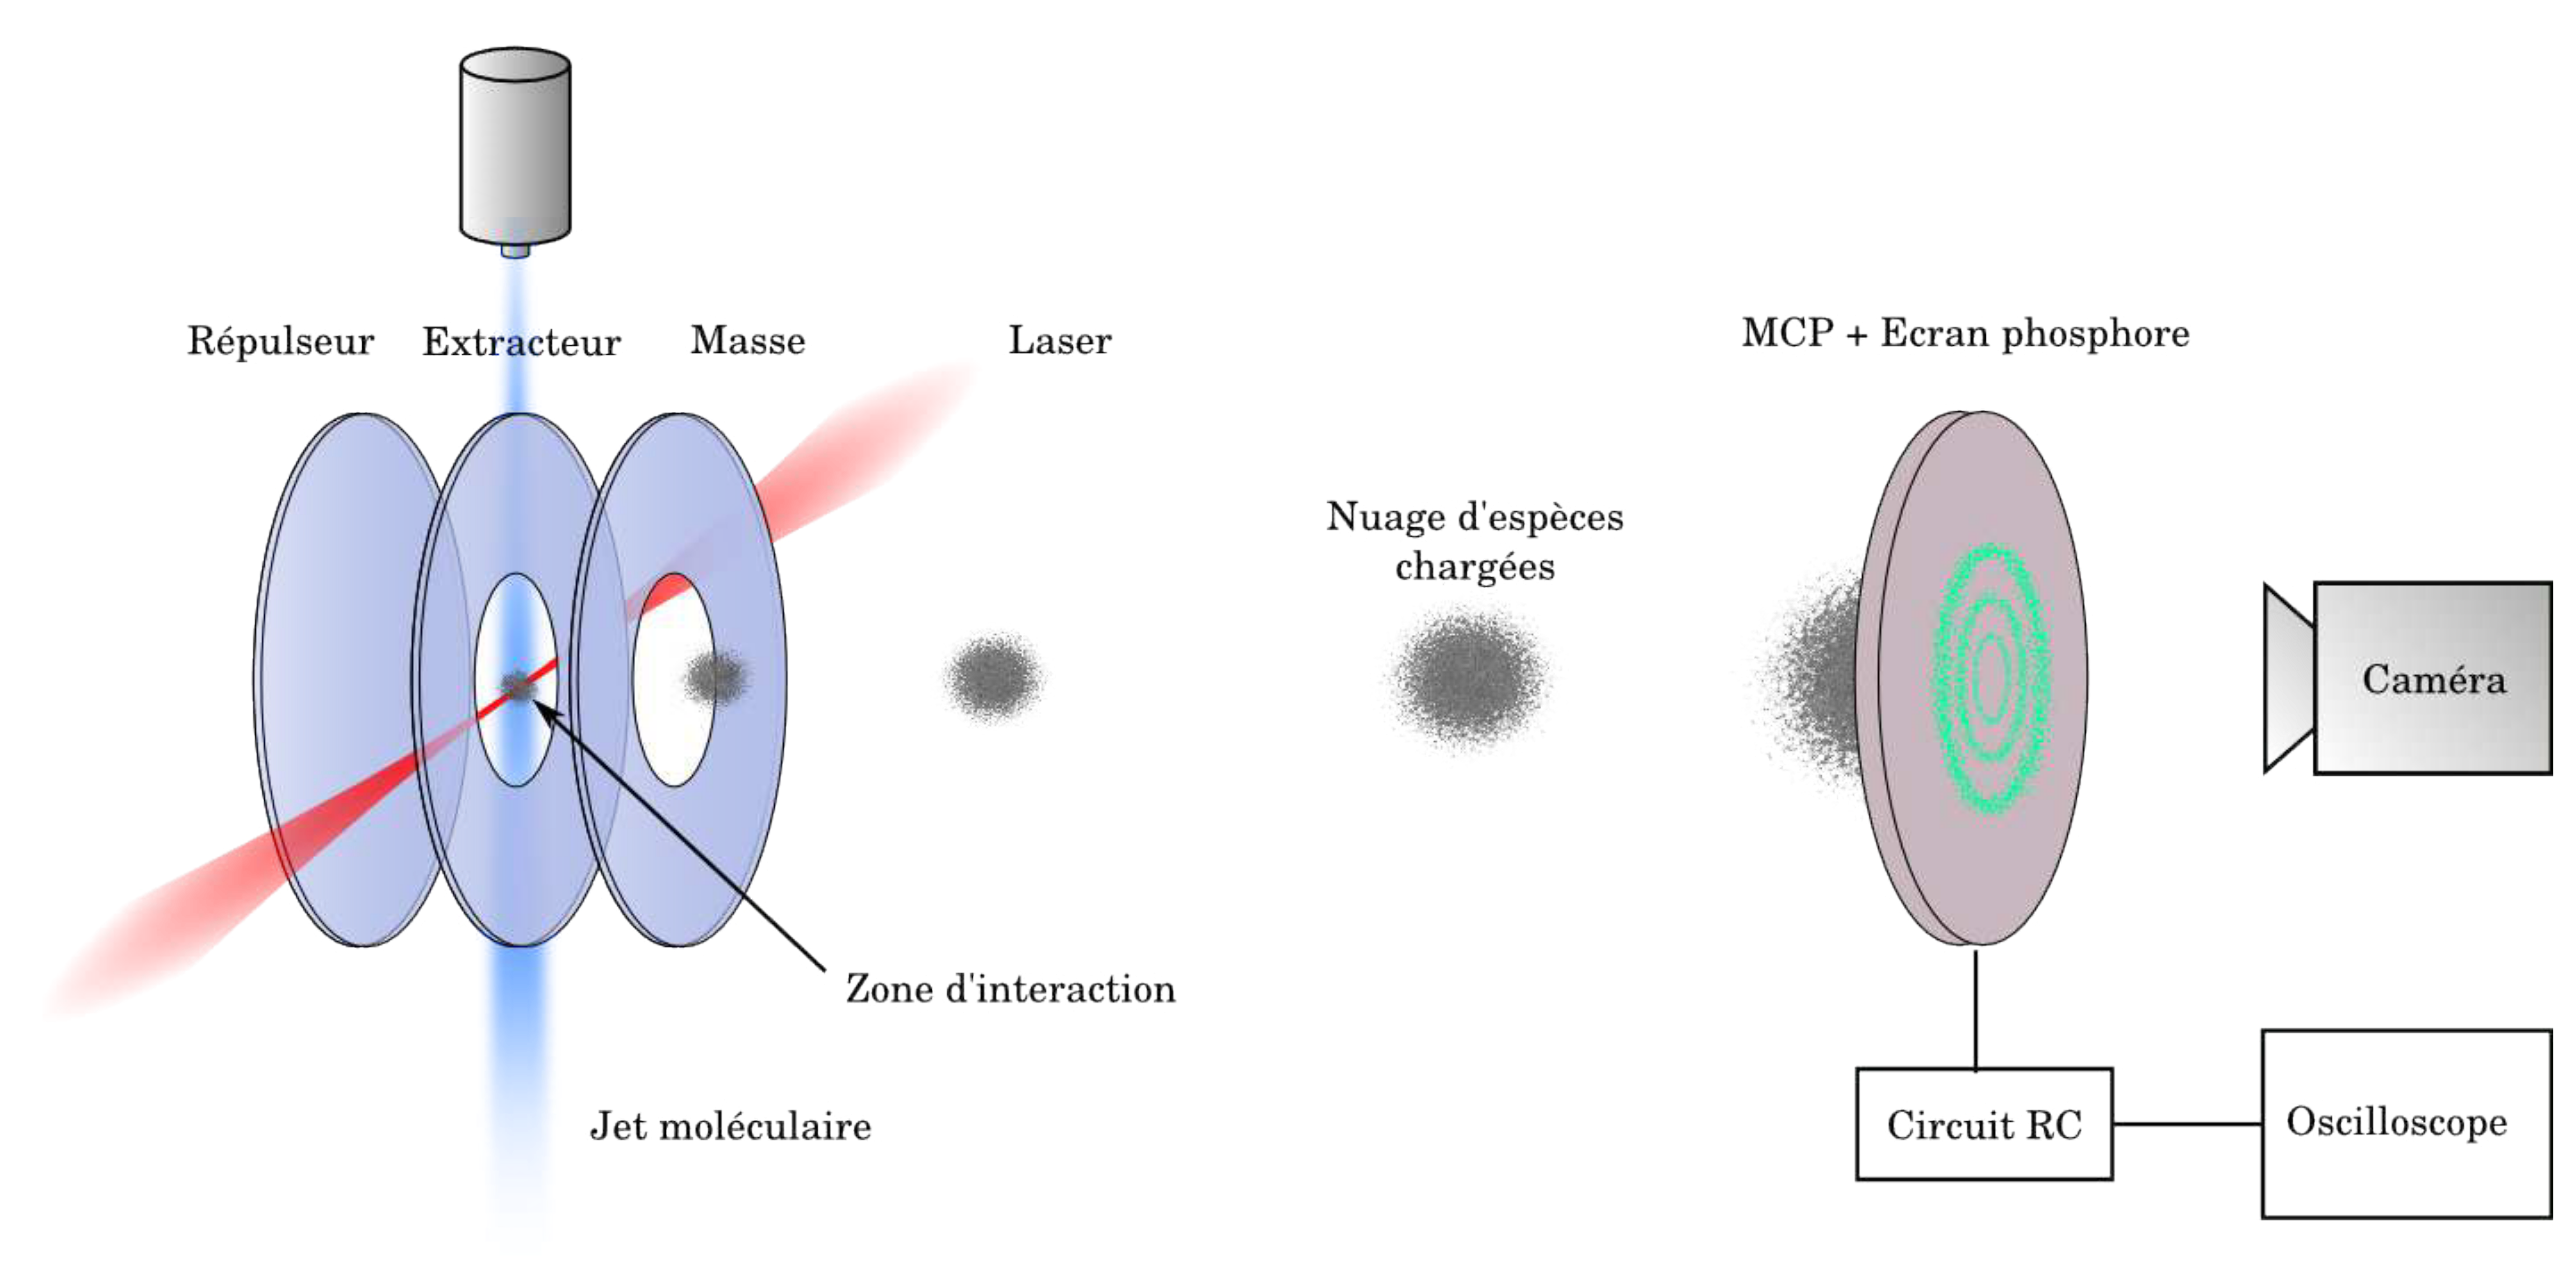
\includegraphics[width=1\columnwidth]{Figures/PECD/vmi.png}%
\caption{Schéma représentatif du fonctionnement d'un VMI (Spectromètre imageur de vecteur vitesse). Tiré de \mycite{handschin}.}
\label{fig:vmi}
\end{figure}

Les deux dernières électrodes de l'appareil sont percées en leur centre, amélioration majeure proposée par \mycite{EppinkParker1997}. L'instrument ainsi réalisé possède des propriétés remarquables. D'abord, les particules sont collectées dans un angle solide avoisinant les $4\pi$ stéradians. De plus, quand la lentille électrostatique est optimisée, toutes les particules de même vecteur vitesse sont focalisées en un unique point du détecteur, quelque soit le lieu où elles ont été émises. C'est cette propriété qui donne son nom à ce spectromètre de vecteur vitesse. On trouvera une discussion très détaillée sur la conception de cet appareil dans la thèse de C. Handschin \mycite{handschin}.

\section{Résultats dans la fenchone}
\label{sec:results_fenchone}
Nous choisissons un système déjà étudié sur synchrotron : la molécule de fenchone ($\text{C}_{10}\text{H}_{16}\text{O}$). Elle possède deux énantiomères, représentés sur la figure \ref{fig:fenchone}. On notera Fenchone (+) l'énantiomère de nom systématique  (1S,4R)-1,3,3-triméthylbicyclo[2.2.1]heptan-2-one et Fenchone (-) l'énantiomère (1R,4S)-1,3,3-triméthylbicyclo[2.2.1]heptan-2-one. L'orbitale moléculaire la plus haute occupée (HOMO) est d'énergie $\simeq$8.6 eV. Les suivantes sont HOMO-1 (10.4 eV), HOMO-2 (10.7 eV), HOMO-3 (11.2 eV), etc. Les valeurs de potentiel d'ionisation ont été obtenus expérimentalement sur synchrotron \mycite{PowisCPC2008}. On voit donc que la troisième harmonique, d'énergie 9 eV, est suffisante pour ioniser la HOMO.

\begin{figure}[!ht]
\centering
\def\svgwidth{0.7\columnwidth}
\import{Figures/PECD/}{fenchone.pdf_tex}
\caption{\'{E}nantiomères de la molécule de fenchone.}
\label{fig:fenchone}
\end{figure}

Pour la mesure de PECD, nous avons utilisé un VMI initialement développé par Valérie Blanchet et Charles Handschin. Un réservoir rempli d'un des deux énantiomères (fourni par Sigma-Aldrich, pureté énantiomérique $\simeq$99\%) est connecté à une buse métallique chauffée à 120\degres C de 300 $\si{\micro\metre}$ de diamètre, placée à 7 cm de la zone d'interaction. 

\begin{figure}[!ht]
\centering
\def\svgwidth{0.8\columnwidth}
\import{Figures/PECD/}{Setup_pecd.pdf_tex}
\caption{Principe de mesure de PECD avec une source d'harmoniques elliptiques.}
\label{fig:pecdsetup}
\end{figure}

La figure \ref{fig:pecdsetup} illustre le principe de l'intégralité du dispositif de mesure de PECD. On alterne successivement polarisation elliptique droite et gauche, en accumulant à chaque fois le signal pendant une dizaine de minutes. On fait ensuite la moyenne de toutes les images obtenues pour chaque polarisation, pour obtenir les grandeurs $I^{1}(r,\theta)$ et $I^{-1}(r,\theta)$, en reprenant les notations de la partie \ref{sec:PECD}. L'approche la plus directe consiste à calculer un paramètre d'asymétrie de Kuhn (voir équation \ref{eq:kuhn}) :
\[g(r,\theta) = 2\frac{I^{1}(r,\theta)-I^{-1}(r,\theta)}{I^{1}(r,\theta)+I^{-1}(r,\theta)}\]

On obtient alors l'image présentée en figure \ref{fig:asym_diff}. Les images des deux énantiomères sont presque parfaitement miroirs l'une de l'autre, ce qui valide la technique de mesure et démontre la qualité de notre source harmonique. Sur une image VMI, la coordonnée radiale $r$ est relié à l'énergie des photoélectrons détectés par une loi de la forme $E = a_0 r^2$. La constante $a_0$ est déterminée en mesurant la section efficace d'une espèce connue, dans notre cas l'argon. Cette constante dépend des tensions appliquées aux électrodes, c'est-à-dire de la focale de la lentille électrostatique du VMI. L'énergie maximale mesurable est donc déterminée par cette focale ainsi que par la taille du détecteur. 

\begin{figure}[!ht]
\centering
\def\svgwidth{0.8\columnwidth}
\import{Figures/PECD/}{asym_diff.pdf_tex}
\caption{Mesure de l'asymétrie avant-arrière pour les deux énantiomères de la fenchone étudiés. Extrait de \mycite{ferre}.}
\label{fig:asym_diff}
\end{figure}

Sur la figure \ref{fig:asym_diff}, on observe un pic d'asymétrie très fort ($\simeq$5\%) proche du centre, c'est-à-dire correspondant à des photoélectrons d'énergie faible. On distingue ensuite trois anneaux concentriques supplémentaires d'énergie plus élevée. Ces différents anneaux correspondent à des photoélectrons provenant de différentes orbitales moléculaires et/ou ionisés par des harmoniques différentes. On observe des inversions de signe entre les anneaux, résultat de la sensitivité du PECD aux états liés (i.e. orbitale ionisé) et aux états du continuum (i.e. à l'énergie de photon utilisée). 

On désire désormais extraire le paramètre $b_1(r)$ (équivalent à $b_1(E)$), ayant montré qu'il portait de nombreuses informations sur le potentiel moléculaire (voir partie \ref{sec:PECD}). Remarquons pour commencer qu'on utilise une galette de micro-canaux, détecteur à deux dimensions, pour mesurer une distribution de vecteur vitesse tridimensionnelle. Par exemple, si on suppose que les photoélectrons de même énergie sont émis de façon isotrope, on a une sphère 3D autour de la molécule ionisée, appelée sphère de Newton. Les différentes contributions donneront différentes sphères concentriques. La figure \ref{fig:sphere_projection} illustre la projection de ces sphères selon la dimension verticale $y$ ($z$ est l'axe optique et $x$ est l'axe du VMI). On voit que la projection est bien plus importante aux pôles qu'à l'équateur de la sphère. 

\begin{figure}[!ht]
\centering
\def\svgwidth{0.6\columnwidth}
\import{Figures/PECD/}{sphere_projection.pdf_tex}
\caption{Projection d'une sphère 3D sur un détecteur 2D. Une coupe selon l'axe $y$ de l'image 2D est tracée.}
\label{fig:sphere_projection}
\end{figure}

Pour passer de la figure 2D à la distribution 3D, on peut appliquer une transformée d'Abel inverse \mycite{heck1995}. Cette transformée requiert d'avoir une symétrie de révolution autour d'un axe contenu dans le plan du détecteur, ce qui est le cas de l'axe optique si on a une polarisation purement circulaire. Nous supposons donc que la polarisation du rayonnement est quasi-circulaire et utilisons un algorithme permettant de réaliser ce traitement de manière efficace, appelé pBasex \mycite{GarciaNahonPowis2004}. L'image \ref{fig:asym_diff} a été analysée en utilisant cette méthode par Gustavo A. Garcia et Laurent Nahon, ce qui dans l'approximation d'un rayonnement quasi-circulaire permet d'extraire $b_1(E)$. Le résultat est présenté sur la figure \ref{fig:pecdfenchone}, où on a noté $\text{PECD}(E) = 2b_1(E)$.

\begin{figure}[!ht]
\centering
\def\svgwidth{1\columnwidth}
\import{Figures/PECD/}{pecdfenchone.pdf_tex}
\caption{PECD mesuré dans la fenchone (+) (pointillés rouges) et (-) (traits bleus) par une source d'harmoniques produites dans \sf6par un champ à 400 nm avec $\epsilon_0=0.3$. Les lignes verticales montrent les différentes orbitales ionisés par les trois harmoniques utilisées.}
\label{fig:pecdfenchone}
\end{figure}

Dans cette figure, on observe différents maxima d'asymétrie, le premier à une énergie d'environ $3\hbar\omega - E_{HOMO}= 0.7$ eV. Les suivants sont environ à $5\hbar\omega - E_{HOMO-1}= 5.1$ eV, $5\hbar\omega - E_{HOMO}= 6.9$ eV, $7\hbar\omega - E_{HOMO-1}= 11.3$eV et $7\hbar\omega - E_{HOMO}= 13.1$ eV. Ces positions sont repérées par les pointillés verticaux. De manière intéressante, le PECD a un signe différent selon l'orbitale ionisée, ce qui est en accord avec des mesures synchrotron \mycite{PowisCPC2008} et met en avant la sensibilité du PECD. Le PECD prend des valeurs très importantes pour l'harmonique 3, ce qui peut être signe d'une très forte ellipticité. Malheureusement aucune mesure de polarimétrie optique n'a été réalisée sur cette harmonique faute de bande passante suffisante du détecteur. La question de l'état de polarisation du rayonnement sera abordée dans la partie suivante.

En conclusion, ces mesures démontrent la possibilité de mesurer un PECD à partir d'une source harmonique. Nous avons récemment étudié le phénomène de PECD dans d'autres régimes d'ionisation. En plus du régime d'ionisation à un photon présenté ici, nous avons mesuré le PECD de la fenchone en ionisation multi-photonique, en ionisation au-dessus du seuil et en ionisation tunnel. Le but est ici de démontrer l'universalité du phénomène de PECD et de montrer la complémentarité des informations obtenues dans les différents régimes d'ionisation. Nous avons de plus cherché à fournir un modèle physique commun à tous les régimes. Ces travaux font l'objet de l'article \ref{pap:BeaulieuNJP2016}, disponible à la fin du manuscrit.

Nous terminerons cette partie par une autre vision du PECD : à la place d'effectuer la spectroscopie d'une molécule grâce à la lumière, nous allons chercher à caractériser l'état de polarisation du rayonnement harmonique grâce à une molécule chirale.

\chapter{Le PECD comme outil de caractérisation du rayonnement}
\section{Le PECD en polarisation elliptique}
Jusqu'à présent, nous avons décrit le PECD en supposant que le rayonnement harmonique était quasi-circulaire. Ce n'est pas exact pour trois raisons :

\begin{itemize}
\renewcommand{\labelitemi}{$\bullet$}
\setlength\itemsep{1em}
\item L'ellipticité de chaque harmonique $\epsilon_q$ n'est pas égale à 1, comme le montrent les mesures optique de la figure \ref{fig:sf6_ell}, qui donnent une borne supérieure $\epsilon_q^{max}<1$. En terme de paramètres de Stokes, cela signifie $s_3<1$.
\item L'ellipse de polarisation du rayonnement produit par la GHOE résonante n'est pas verticale : comme le montre la figure \ref{fig:antoinepra}, l'ellipse est tournée d'un angle $\eta$ qui augmente avec l'ellipticité du fondamental $\epsilon_0$. On a donc à la fois $s_1$ et $s_2\neq 0$.
\item Le rayonnement n'est pas complètement polarisé : on a un degré de polarisation $P<1$. La valeur de $s_3$ est alors diminuée : $s_3 \rightarrow Ps_3$.
\end{itemize}


Nous devons calculer la distribution angulaire de photoélectron produite par ce rayonnement imparfait. Pour ce faire, il faut calculer la section différentielle de photoionisation dans le référentiel du laboratoire. Nous reprenons les notations de la partie \ref{sec:PECD}, où les coordonnées sphériques $(r,\theta,\phi)$ sont définies sur la figure \ref{fig:geomPECD}. Le calcul complet de la section différentielle de photoionisation dans ce cas est réalisé dans l'annexe de \mycite{ferre}. Elle est ensuite exprimée en fonction des paramètres de Stokes du rayonnement. L'expression finale est :
\begin{align}
\frac{\rmd\sigma^p}{\rmd\Omega_{\vec{k}}}(r,\theta,\phi) &\propto b_0^p(r)+s_3b_1^p(r)P_1(\cos\theta)+b_2^p(r)P_2(\cos\theta)\\
&+b_2'^p(r)\left[s_1\cos(2\phi)+s_2\sin(2\phi)\right]P_2^2(\cos\theta),
\label{eq:sigma_ell}
\end{align}

où $p=\pm1$ correspond à une polarisation elliptique gauche ou droite. On voit que $s_1$, $s_2$ et $s_3$ interviennent dans cette nouvelle expression. Dans la pratique, la mesure se fait en deux dimensions et intègre donc l'équation \ref{eq:sigma_ell} selon $\phi$. Avec notre convention d'angle, l'élément de volume infinitésimal s'écrit $\rmd V = r\rmd r \rmd \phi \sin\theta \rmd \theta$. Ainsi, l'image 2D obtenue correspond à :
\begin{equation*}
I^p(r,\theta) = \int_{\phi=0}^{2\pi}\frac{\rmd\sigma}{\rmd\Omega_{\vec{k}}}(r,\theta,\phi)\rmd\phi,
%\label{eq:sigma_ell}
\end{equation*}
On peut réécrire le terme de l'équation \ref{eq:sigma_ell} dépendant de $\phi$. On a (équation \ref{eq:stokes2}) :
\begin{align*}
s_1 &= Ps_0\cos 2\chi\cos 2\eta ,\\
s_2 &= Ps_0\cos 2\chi\sin 2\eta,
\end{align*}
où on rappelle que $\eta$ est l'angle de l'ellipse par rapport au repère cartésien, et l'ellipticité vaut $\epsilon=\tan\chi$. On réécrit donc :
\begin{align*}
\left[s_1\cos(2\phi)+s_2\sin(2\phi)\right] &= PS_0\cos 2\chi\left[\cos(2\eta)\cos(2\phi)+\sin(2\eta)\sin(2\phi)\right]\\
&= PS_0\cos 2\chi \cos(2(\phi+\eta)).
\end{align*}
Si on a une polarisation circulaire pure, $\epsilon = 1 = \tan\chi$, donc $\cos2\chi = 0$. Le terme en $b_2'$ est donc non nul seulement pour une polarisation elliptique. De plus, son intégrale selon $\phi$ s'annule. On retrouve donc l'image 2D mesurée expérimentalement :
\begin{equation*}
I^p(r,\theta) = \int_{\phi=0}^{2\pi}\frac{\rmd\sigma}{\rmd\Omega_{\vec{k}}}(r,\theta,\phi)\rmd\phi = b_0^p(r)+s_3b_1^p(r)P_1(\cos\theta)+b_2^p(r)P_2(\cos\theta),
\end{equation*}
On peut donc toujours calculer $\text{PECD} = I^1-I^{-1} = 2s_3b_1P_1(\cos\theta)$. Par contre, le terme dépendant de $\phi$ dans la section différentielle de photoionisation vient quand même briser la symétrie autour de l'axe optique. Cette brisure de symétrie est illustrée dans la figure \ref{fig:sphere_ell}. On y trace des isosurfaces de $\rmd\sigma/\rmd\Omega$, où on a choisi un profil gaussien de $b_0$, centré sur une énergie qui correspondrait à celle du photoélectron. Cette discussion ne concernant pas $b_2$, on le choisi nul, tandis que $b_1$ et $b_2'$ sont pris proportionnels à $b_0$. Leurs coefficients de proportionnalité sont choisis volontairement bien plus importants que dans un cas réel pour accentuer leurs effets. On voit que pour une polarisation linéaire, la distribution est isotrope. Pour une polarisation circulaire, elle est plus dirigée vers l'avant. Quand on considère une polarisation elliptique, on a une distribution plus complexe, non symétrique selon $\phi$ et qui dépend de $\eta$.

\begin{figure}[!ht]
\centering
\def\svgwidth{1\columnwidth}
\import{Figures/PECD/}{sphere_ellipse.pdf_tex}
\caption{Isosurfaces de la section efficace différentielle de photoionisation, pour une polarisation linéaire, circulaire et elliptique avec un angle de l'ellipse $\eta=0,\;45,\;90,\;135$\degres.}
\label{fig:sphere_ell}
\end{figure}

En conclusion, les hypothèses nécessaires à l'application des techniques usuelles d'inversion, comme pBasex, ne sont pas vérifiées. Cet algorithme ne donnera une valeur exacte que dans le cas d'une polarisation parfaitement circulaire. En particulier, il introduira un artefact sur la valeur de $b_0$, le spectre de photoémission. Par contre, $b_1$ peut toujours être retrouvé dans la différence $I^1-I^{-1}$. Pour effectuer une normalisation et exprimer $b_1$ en pourcentage, il faudrait diviser cette différence par $b_0$ mesuré en polarisation linéaire, comme suggéré dans le chapitre 5 de \mycite{ferre}.

Une fois ces précautions prises, on voit que le PECD dépend linéairement de $s_3$. En tant que phénomène chiroptique, le PECD est sensible à la \textit{vraie} ellipticité du rayonnement, contrairement aux méthodes optiques utilisées jusqu'à présent. On a donc la possibilité de caractériser complètement l'état de polarisation du rayonnement harmonique grâce au PECD. Pour ce faire, trois mesures sont nécessaires :
\begin{itemize}
\renewcommand{\labelitemi}{$\bullet$}
\setlength\itemsep{1em}
\item Une mesure de PECD de référence sur une source ayant $s_3 = 1$ et $P = 1$ à la même énergie de photon. 
\item Une mesure utilisant la source harmonique. Le rapport des PECD avec la mesure précédente donnera sa valeur de $s_3$.
\item Une mesure de loi de Malus sur la source harmonique dans les mêmes conditions, qui donnera $s_1$, $s_2$ et la borne supérieure de l'ellipticité. Le rapport entre cette borne supérieure et la véritable ellipticité donnera la valeur de $P$.
\end{itemize}
\vspace{12pt}
L'élément manquant est donc la mesure de référence sur une source complètement polarisée. Des études précédentes donnent des valeurs pour le PECD de la fenchone (\mycite{PowisCPC2008}) mais pas dans la gamme spectrale correspondant à notre spectre harmonique, en particulier aux énergies de photon faibles ($E_{H3} = 9.3$ eV). Ceci a motivé une campagne d'expériences au synchrotron SOLEIL en Février 2015, dont il est question dans la partie suivante.

\section{Mesures de référence sur synchrotron}
\subsection{La ligne DESIRS au synchrotron SOLEIL}
Sur un synchrotron, des paquets d'électrons sont d'abord accélérés dans un accélérateur linéaire avant de passer dans un onduleur, qui génère un champ magnétique perpendiculaire à la trajectoire des électrons. Le champ magnétique crée une oscillation du paquet d'électrons, qui s'accompagne d'une émission de lumière appelée rayonnement synchrotron. En jouant sur les paramètres des électrons, on peut modifier ceux de la lumière générée. Ainsi, il est possible d'obtenir un rayonnement ultra-violet intense et complètement accordable en énergie. De plus, si on applique des champs magnétiques différents selon les axes $x$ et $y$, on peut créer des oscillations selon chaque direction déphasées entre elles. On peut ainsi contrôler la polarisation de la lumière émise.

Nous avons réalisé une campagne sur la ligne DESIRS du synchrotron SOLEIL \mycite{NahonJSR2012}, ligne construite pour la spectroscopie et la mesure de dichroïsmes avec une haute résolution en énergie. Elle fournit un rayonnement d'énergie 5 à 40 eV, qui est sélectionné spectralement par une série de 4 réseaux de diffraction, permettant d'atteindre jusqu'à $\SI{54}{\micro\eV}$ de résolution à 13 eV.

Sur la ligne DESIRS, la polarisation de la lumière est contrôlée à l'aide de l'onduleur électromagnétique OPHELIE, représenté sur la figure \ref{fig:onduleur}. Les deux onduleurs croisés peuvent être translatés l'un par rapport à l'autre, de sorte à avoir un déphasage variable entre -90\degres et 90\degres. Les courants sont également ajustables pour contrôler l'amplitude des champs magnétiques appliqués. Pour la spectroscopie, il est important de caractériser l'état de polarisation de la lumière émise. Il peut varier à cause d'imperfections de l'onduleur, de la géométrie de la ligne optique, ou de dépôts sur les optiques utilisées. Pour ce faire, la ligne DESIRS est équipée d'un polarimètre VUV permettant de caractériser complètement l'état de la lumière, y compris le degré de polarisation \mycite{NahonAO2004}. Ce polarimètre est placé après un monochromateur et utilise 6 réflexions sur des prismes qui déphasent et analysent l'état du champ. Ce dispositif est unique au monde et est très efficace lorsqu'on dispose d'un flux tel que celui d'un synchrotron. Les paramètres de l'onduleur ont ainsi été optimisés jusqu'à obtenir des performances remarquables : le champ polarisé circulairement droit vérifie en moyenne $s_3/s_0=92.1\pm2.3$\% tandis que le polarisé circulairement gauche a $s_3/s_0=95.2\pm2.9$\% \mycite{NahonAO2004}.

\begin{figure}[!ht]
\centering
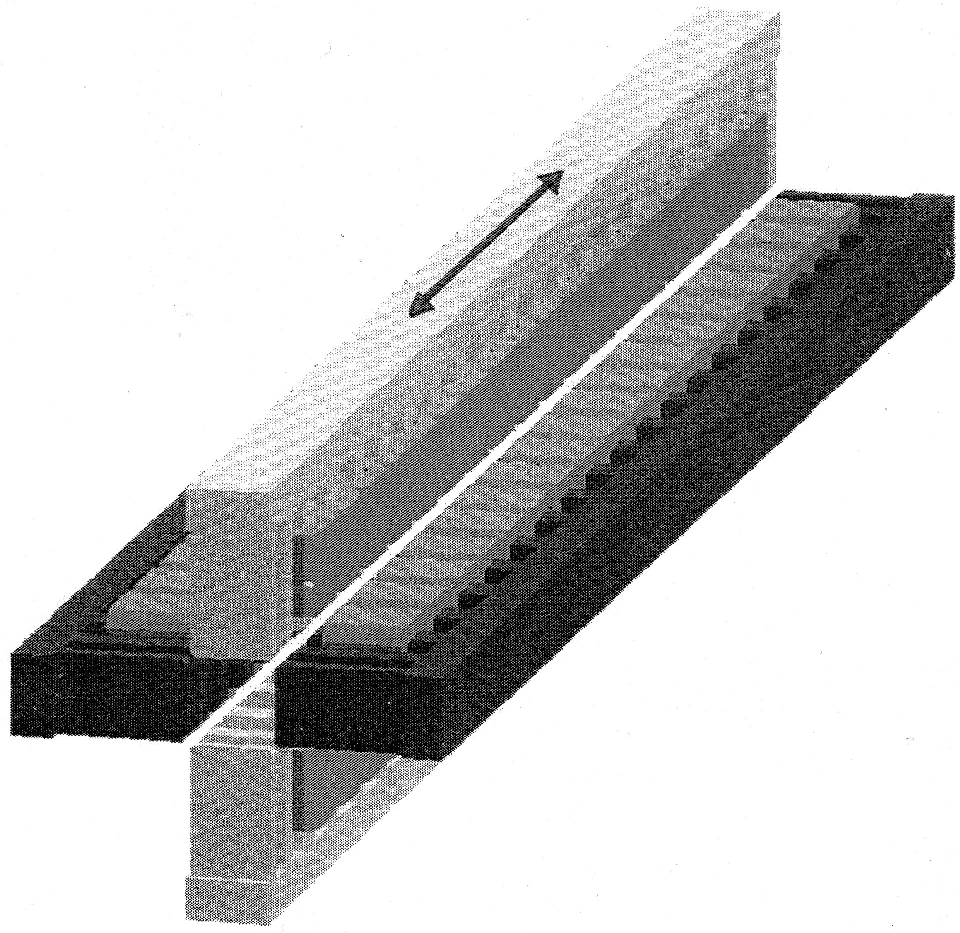
\includegraphics[width=0.4\columnwidth]{Figures/Soleil/onduleur.jpg}%
\caption{Schéma de l'onduleur croisé OPHELIE. Un onduleur peut être translaté par rapport à l'autre, permettant d'ajuster le déphasage entre les deux composantes de la lumière émise. Tiré de \mycite{NahonAO2004}.}
\label{fig:onduleur}
\end{figure}

Pour la mesure de PECD, le polarimètre est retiré et le champ est envoyé dans la zone d'interaction du spectromètre VMI Delicious. Ce spectromètre est amélioré par rapport à celui présenté plus haut car il est capable de mesurer à la fois la distribution de vecteur vitesse des électrons et le temps de vol des ions créés par le champ VUV. Le temps de vol donne la masse des ions, ce qui permet d'effectuer une analyse de corrélation et de sélectionner les électrons provenant d'une espèce donnée. On résout également les différents rapports de branchement de l'espèce chirale, même si nous ne nous sommes pas encore intéressés à cette quantité.

\subsection{Comparaison entre PECD en polarisation elliptique ou circulaire}
Commençons par étudier expérimentalement l'effet d'une polarisation elliptique sur la mesure de PECD. Comme expliqué plus haut, la polarisation du rayonnement synchrotron est modifiée en ajustant les paramètres de l'onduleur puis mesurée par le polarimètre VUV. On se place à une énergie de photon de 9.3 eV (énergie de la troisième harmonique dans la mesure réalisée au CELIA), et on choisit un rayonnement purement circulaire ou bien elliptique. Le champ elliptique a les paramètres de Stokes suivants :
\[ s_1=0.53\quad s_2=0.03\quad s_3=0.82, \]
ce qui correspond à une ellipse de polarisation tournée de $\eta=1.61$\degres~et d'ellipticité $\epsilon = 0.54$ (voir formules \ref{eq:stokes2inv}), tracée plus bas sur la figure \ref{fig:circ_ell_b0} .
 
On utilise un jet de fenchone (Sigma Aldrich). \`{A} cette énergie de photon, seule l'orbitale HOMO, d'énergie 8.6 eV, peut être ionisée. La figure \ref{fig:circ_ell_b0} présente le $b_0$ (spectre de photoémission) obtenu avec le rayonnement circulaire et elliptique. Le traitement utilise ici l'agorithme pBasex. L'échelle horizontale utilisée est l'énergie d'ionisation, définie comme $E_I = \hbar\omega - E_{\text{\'electron}}$. Les profils de $b_0$ sont remarquablement similaires. Leur amplitude est légèrement différente mais on rappelle que, pBasex ayant été utilisé, la valeur absolue de $b_0$ n'est pas correcte dans le cas elliptique.

\begin{figure}[!ht]
\centering
\def\svgwidth{0.8\columnwidth}
\import{Figures/Soleil/}{Circ_Ell_b0.pdf_tex}
\caption{Mesures de $b_0$ dans la fenchone réalisées sur la ligne DESIRS à une énergie de photon de 9.3 eV. En traits pleins, polarisation circulaire. En pointillés, polarisation elliptique. Les deux ellipses de polarisation correspondantes sont tracées à droite de la figure.}
\label{fig:circ_ell_b0}
\end{figure}

Sur la figure \ref{fig:circ_ell_b1} est représenté le paramètre dichroïque $b_1$ dans les cas circulaire et elliptique. On étudie ici la valeur de $b_1$ non normalisée par $b_0$, c'est-à-dire la simple différence $I^1-I^{-1}$. Les données pour le cas circulaire ont été prises dans la fenchone (+), tandis que celles du cas elliptique dans la fenchone (-). On a donc tracé $-b_1^{\text{circ}}$ et $b_1^{\text{ell}}$. En changeant d'énantiomère, on doit normalement mesurer une inversion parfaite de $b_1$. Au cours de cette campagne, nous avons observé une différence systématique entre les deux énantiomères. Une étude plus poussée, qui fait l'objet de l'article \ref{pap:NahonPCCP2016} \mycite{NahonNagGarciaEtAl2016}, a montré que cette différence était due à une différence de pureté énantiomérique des échantillons. Si l'échantillon de fenchone (+) était énantiopur à 99\%, celui de fenchone (-) ne l'était qu'à 82\%. Dans cette étude nous démontrons la possibilité de mesurer l'excès énantiomérique grâce au PECD avec une précision de $\pm1$\%. $b_1^{\text{ell}}$ ainsi que toutes les autres données dans la fenchone (-) ont donc été corrigées en fonction.

\begin{figure}[!ht]
\centering
\def\svgwidth{0.8\columnwidth}
\import{Figures/Soleil/}{Circ_Ell_b1.pdf_tex}
\caption{Mesures de $b_1$ dans la fenchone (-) pour des polarisations circulaires et elliptiques. Les barres d'erreurs sont issues d'une analyse statistique.}
\label{fig:circ_ell_b1}
\end{figure}

On voit que là où le signal est significatif (entre $\simeq8.5$ et $\simeq 9$ eV), les deux courbes de $b_1$ sont très ressemblantes, à un facteur de proportionnalité près. Sur la largeur à mi-hauteur du pic, on mesure $b_1^{\text{ell}}/b_1^{\text{circ}} = 0.83 \pm 0.03$. Rappelons qu'on a mesuré $s_3^{\text{ell}} = 0.82$ et que la ligne fournit en moyenne $s_3^{\text{circ}} \simeq 1$. Le PECD évoluant linéairement en $s_3$, on s'attend donc à une valeur théorique de $b_1^{\text{ell}}/b_1^{\text{circ}} \simeq 0.82$, ce qui est tout à fait dans notre intervalle de confiance. Nous avons donc vérifié expérimentalement la dépendance du PECD pour une polarisation imparfaite telle que celle du rayonnement harmonique.

\subsection{Mesures de $b_1$ aux énergies harmoniques}
Nous présentons ici les mesures réalisées aux énergies correspondant aux harmoniques de la source présentée à la partie \ref{sec:sf6ghoe} : 9.3 eV (H3), 15.5 eV (H5) et 21.7 eV (H7). Nous avons également mesuré le PECD de la fenchone aux énergies correspondant à H4 et H6, ainsi que dans la zone 9.3 à 11.5 eV. Ces mesures, non présentées ici, serviront de données de référence pour de futures expériences dans lesquelles on prévoit d'observer des dynamiques vibrationnelles grâce au PECD résolu en temps.

\begin{figure}[!ht]
\centering
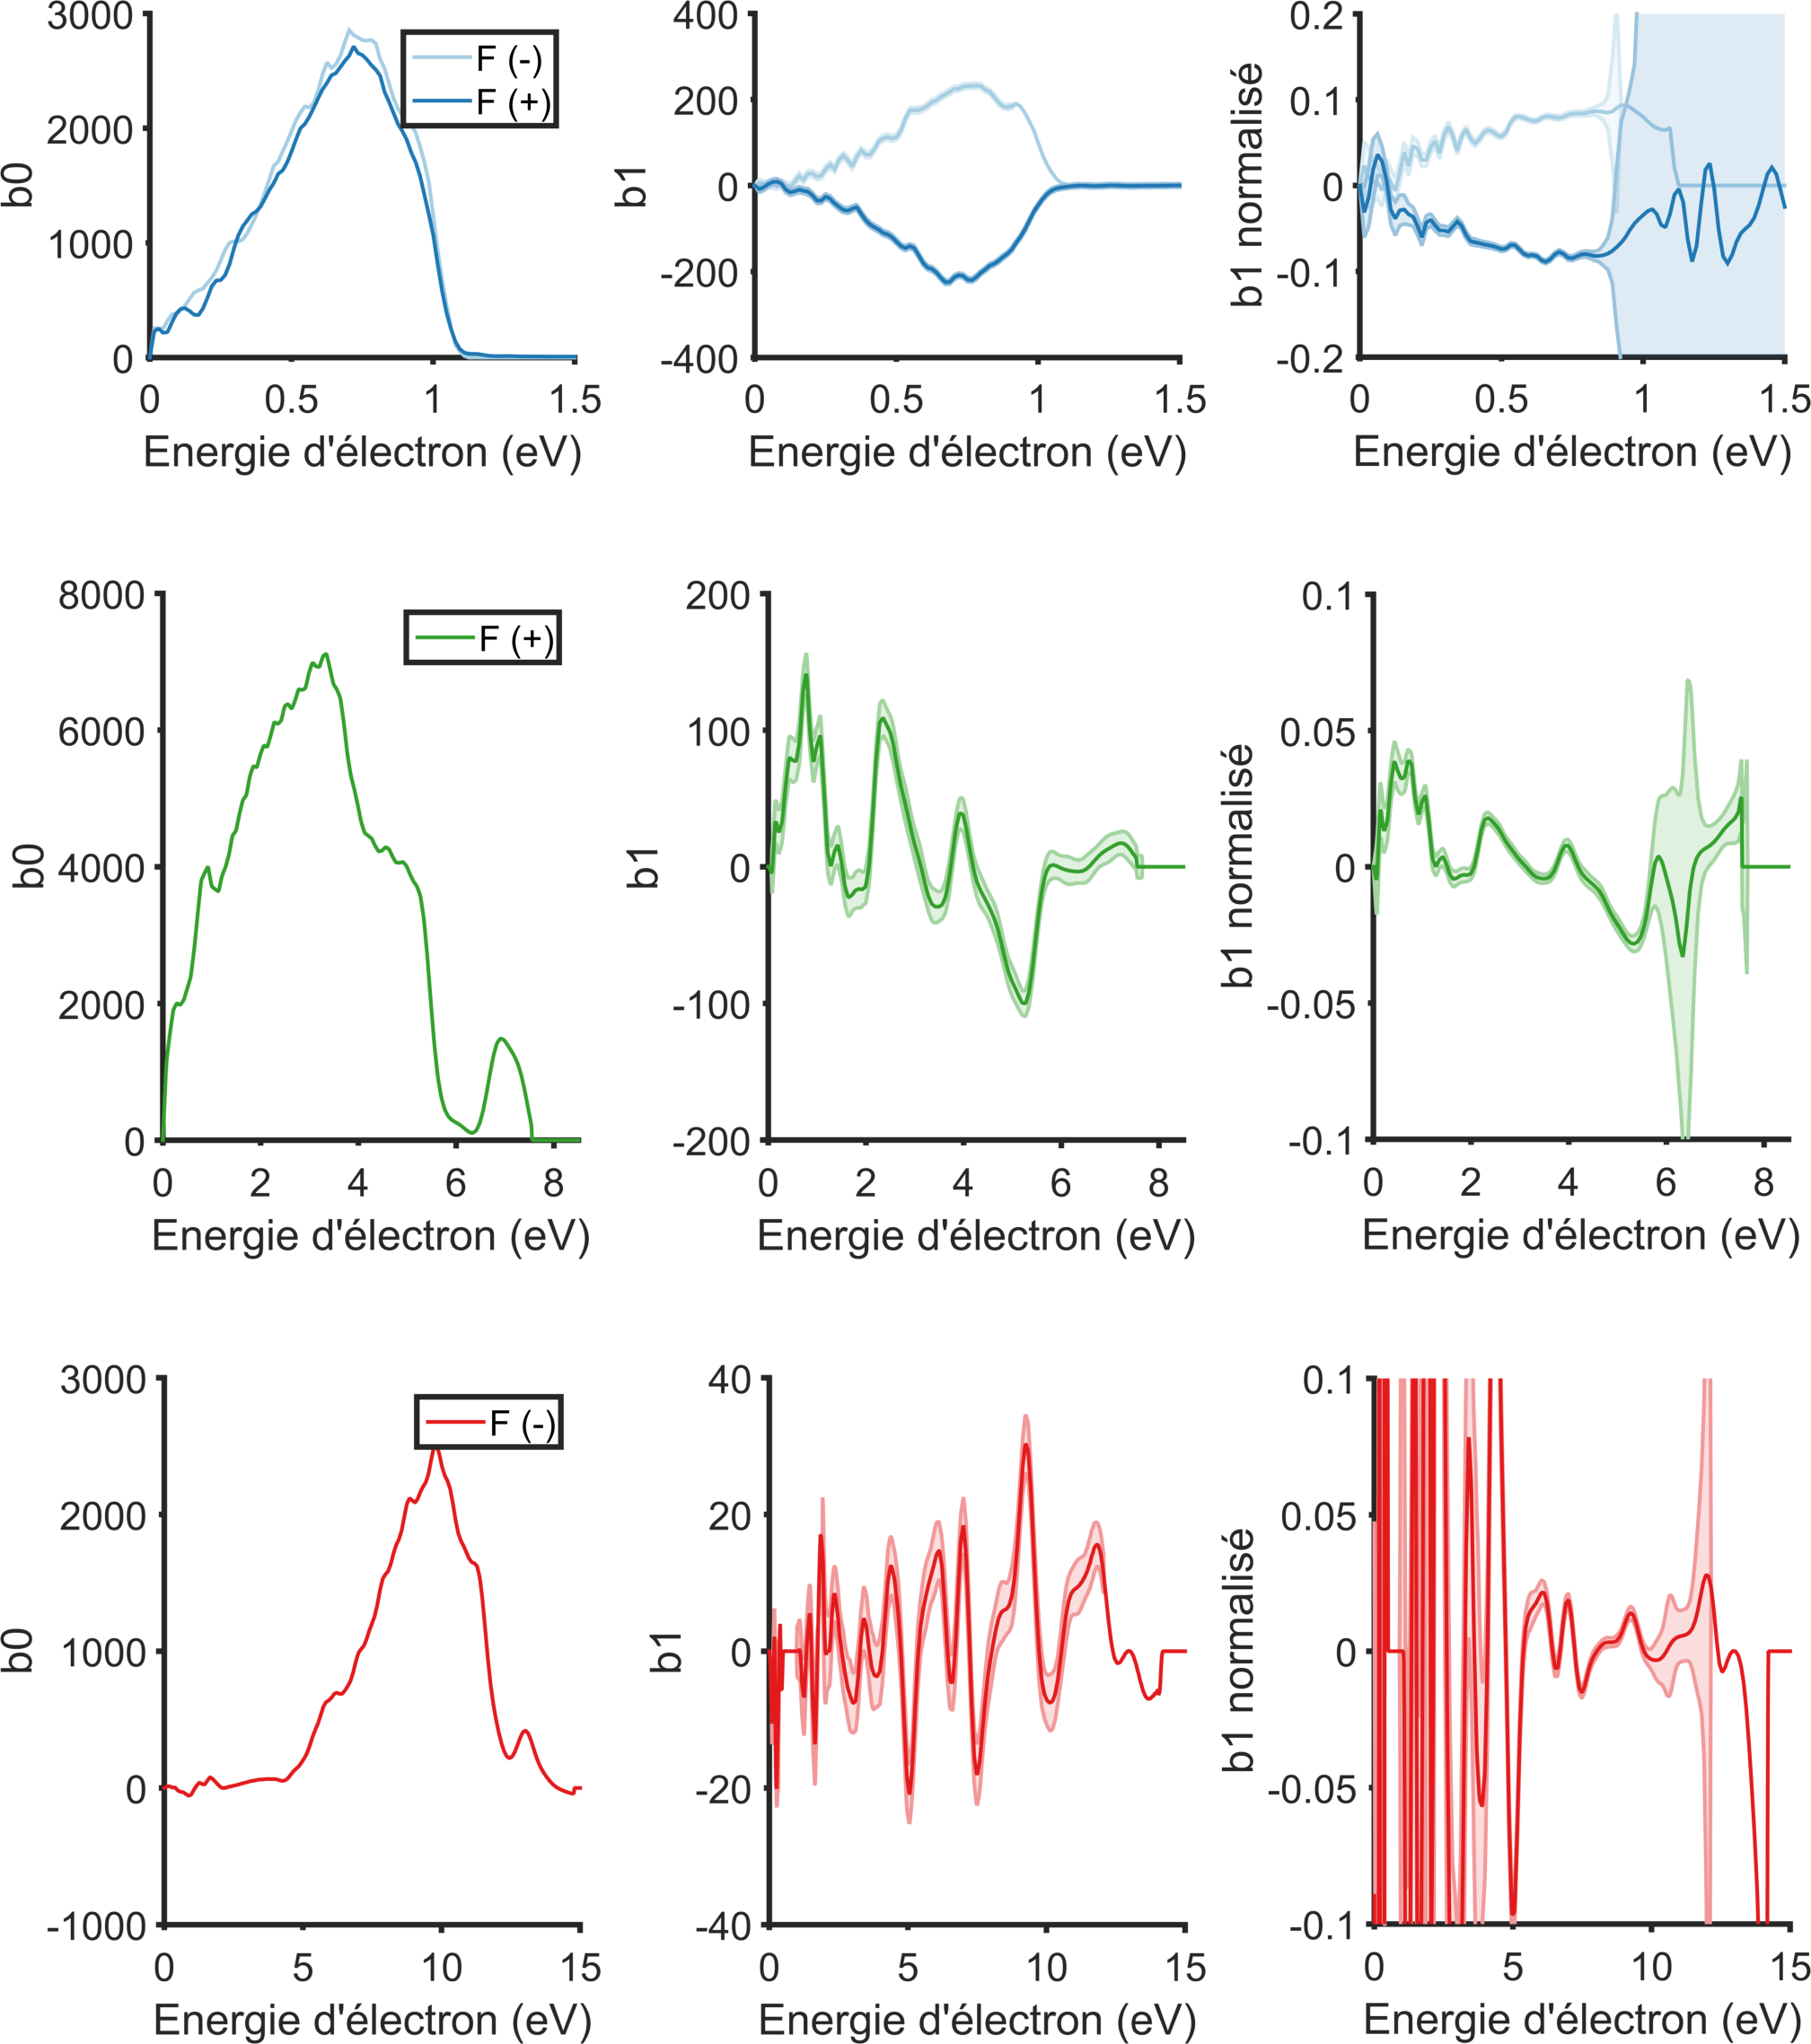
\includegraphics[width=1\columnwidth]{Figures/Soleil/Results_PECD.pdf}%
\caption{Résumé des mesures de PECD réalisées sur la ligne DESIRS. De gauche à droite : $b_0$ (spectre de photoémission), $b_1$, et $b_1$ normalisé par $b_0$. De haut en bas, énergies de photon égales à 9.3 eV, 15.5 eV et 21.7 eV. Pour la première énergie on a tracé la mesure pour les deux énantiomères.}
\label{fig:results_pecd}
\end{figure}

Dans la figure \ref{fig:results_pecd}, on trace $b_0$, $b_1$, et $b_1/b_0$ pour les trois énergies harmoniques et pour un ou deux énantiomère. La polarisation étant ici complètement circulaire, l'utilisation de pBasex est justifiée. Quand on augmente l'énergie de photon, l'énergie maximale de photoélectron observée augmente également. Dans tous les cas, on observe clairement l'ionisation depuis la HOMO, à une énergie égale à $\hbar\omega-I_P^\text{HOMO}$, c'est-à-dire $\simeq \SI{0.7}{eV},\; \SI{6.9}{eV},\text{ et }\SI{13.1}{eV}$ respectivement pour H3, H5 et H7. Pour les énergies de photons plus élevées, la contribution d'orbitales plus basses apparaît. Les énergies de ces orbitales sont de plus en plus proches, et leurs contributions sont sommées dans le $b_1$ observé. $b_1$ est différent pour chacune d'entre elles et peut changer de signe, ce qui explique les profils riches observés dans cette région. Précisons pour terminer qu'à cause de problèmes de calibration en énergie aux hautes énergies de photon, certaines courbes ont été interpolées pour être cohérentes avec potentiels d'ionisation des différentes orbitales publiés dans la littérature \mycite{PowisCPC2008}.
\newpage
\section{Comparaison entre mesures synchrotron et harmoniques}
\label{sec:soleil_vs_celia}
\subsubsection{Formulation mathématique}
Nous dispose désormais des données synchrotron nécessaires à la caractérisation complète de l'état de polarisation du champ harmonique. Toutefois, nous allons voir que nos mesures harmoniques sont incomplètes. Nous illustrerons ici le principe à suivre mais nous pourrons pas donner de véritable valeurs numériques en l'état.

On considère donc le spectre constitué des 3 première harmoniques du fondamental à 400 nm. Quand il ionise la molécule de fenchone, on observe un spectre de photoémission qui est la somme de la contribution de chaque harmonique :
\[ b^{\text{GHOE}}_0(E) = \sum_{q={3,5,7}} s^{\text{GHOE},q}_0 \times b^{\hbar\omega=E_q}_0(E),\]
où $E_q$ et $s^{\text{GHOE},q}_0$ sont respectivement l'énergie et le $s_0$ (= l'intensité) de la q-ième harmonique.

Les trois mesures synchrotrons donnent quant à elles pour $q=3,5,7$ :
\[ b^{\text{Sync},q}_0(E) =  s^{\text{Sync},q}_0 \times b^{\hbar\omega=E_q}_0(E),\]

Notons les inconnues du problème $a_q = s^{\text{GHOE},q}_0/s^{\text{Sync},q}_0$ pour $q=3,5,7.$ On les obtient par un calcul d'ajustement, par exemple au sens des moindres carrés :
\begin{equation}
\min_{a_q} \sqrt{\int_{E=0}^{E_\text{max}} \left(b^{\text{GHOE}}_0(E)-\sum_{q={3,5,7}} a_q \times b^{\text{Sync},q}_0(E)\right)^2\rmd E}.
\label{eq:minb0}
\end{equation}

La figure \ref{fig:sumb0} présente le profil de $\sum_{q={3,5,7}} b^{\text{Sync},q}_0(E)$, en utilisant les $b_0$ mesurés à la partie précédente (voir figure \ref{fig:results_pecd}). Elle permet de voir les régions dans lesquelles contribuent chaque énergie de photon.

\begin{figure}[!ht]
\centering
\def\svgwidth{0.8\columnwidth}
\import{Figures/Soleil/}{sumPES.pdf_tex}
\caption{Sommes des $b_0$ mesurés au synchrotron à chaque énergie harmonique, en les supposant chacun normalisés et de poids égal.}
\label{fig:sumb0}
\end{figure}

De la même manière, le paramètre dichroïque $b_1$ s'écrit pour les harmoniques :
\[ b^{\text{GHOE}}_1(E) = \sum_{q={3,5,7}} s^q_3 s^{\text{GHOE},q}_0 \times b^{\hbar\omega=E_q}_1(E),\]
et pour les mesures synchrotron, où on considère $s_3=1$ :
\[ b^{\text{Sync},q}_1(E) =  s^{\text{Sync},q}_0 \times b^{\hbar\omega=E_q}_1(E).\]

La quantité à minimiser en fonction des trois inconnues $s_3^3,\;s_3^5,\;s_3^7$ est alors :
\begin{equation}
\min_{s_3^q} \sqrt{\int_{E=0}^{E_\text{max}} \left(b^{\text{GHOE}}_1(E)-\sum_{q={3,5,7}} s^q_3 \times a_q \times b^{\text{Sync},q}_1(E)\right)^2\rmd E}.
\label{eq:minb1}
\end{equation}

En pratique, on minimise à la fois les problèmes \ref{eq:minb0} et \ref{eq:minb1} :
\begin{equation}
\min_{a_q,\;s_3^q} \sqrt{
	\begin{aligned}
	\int_{E=0}^{E_\text{max}}&\alpha_0\left(b^{\text{GHOE}}_0(E)-\sum_{q={3,5,7}} a_q \times b^{\text{Sync},q}_0(E)\right)^2 \\
	&+ \alpha_1\left(b^{\text{GHOE}}_1(E)-\sum_{q={3,5,7}} s^q_3 \times a_q \times b^{\text{Sync},q}_1(E)\right)^2	\rmd E
	\end{aligned}
	}
\label{eq:min_total}
\end{equation}
où $\alpha_0$ et $\alpha_1$ sont les poids relatifs qu'on donne arbitrairement à l'ajustement du $b_0$ et du $b_1$. Cette procédure donnera la valeur optimale de $s_3^3,\;s_3^5$ et $s_3^7$, valeurs inaccessible par des méthodes optiques.

\subsubsection{Première application de la méthode}
Pour les données synchrotron, nous choisissons d'utiliser la mesure sur la fenchone (+) pour H5, et sur la fenchone (-) pour H3 et H7 où on inversera le $b_1$. Ces mesures sont les plus précises du fait d'un très bon niveau de signal, et ne présentent pas de problème de calibration. On prend également soin de corriger les mesures dans la fenchone (-) de l'erreur due à l'excès énantiomérique inférieur à 1.

Pour les données harmoniques, les seules dont nous disposons actuellement sont celles présentées sur la figure \ref{fig:pecdfenchone}. Le problème est qu'elles ont été obtenues par application de l'algorithme pBasex, qui introduit un artefact pour une polarisation non circulaire. On peut toujours étudier le $b_1$ non normalisé par $b_0$ (c'est-à-dire la différence directe entre les deux images), mais la formule \ref{eq:min_total} montre bien la nécessité de connaître $b_0$ pour comparer les deux mesures.

En plus de ce problème d'analyse, ces données ne sont pas parfaites : des zones du détecteurs étaient brûlées (visible sur la figure \ref{fig:pecdfenchone} vers 6 eV), et un bruit de fond n'a pas été correctement soustrait. Nous appliquerons donc le calcul présenté plus haut tout en gardant à l'esprit que les valeurs finales seront incorrectes. 

Le problème \ref{eq:min_total} est résolu au sens des moindres carrés par un algorithme à région de confiance réflectif \mycite{BranchColemanLi1999}. On restreint de plus le domaine d'énergie sur lequel on minimise la fonction, de sorte à ne garder que les pics significatifs. $b_1$ étant le paramètre qui nous intéresse le plus, on choisit des facteurs de pondération $\alpha_1/\alpha_0 = 100$. La figure \ref{fig:results_minim_P} illustre le résultat de l'algorithme, qui converge en quelques dizaines d'itérations, pour la fenchone (+). Les $b_1$ des mesures synchrotrons sont ensuite inversés pour analyser le cas de la fenchone (-), illustré sur la figure \ref{fig:results_minim_M}.

\begin{figure}[!ht]
\centering
\def\svgwidth{0.75\columnwidth}
\import{Figures/Soleil/}{results_minim_P.pdf_tex}
\caption{Détermination des $s_3$ harmoniques par comparaison avec les données synchrotron dans la fenchone (+). En traits pleins bleus, résultats de l'algorithme de minimisation. En pointillés rouges, mesures faites avec la source d'harmoniques d'ordre élevé. Les rectangles verts illustrent le domaine d'énergie où a été effectuée la minimisation. Les valeurs de $s_3$ obtenues sont indiquées.}
\label{fig:results_minim_P}
\end{figure}

\begin{figure}[!ht]
\centering
\def\svgwidth{0.75\columnwidth}
\import{Figures/Soleil/}{results_minim_M.pdf_tex}
\caption{Détermination des $s_3$ harmoniques par comparaison avec les données synchrotron dans la fenchone (-). En traits pleins bleus, résultats de l'algorithme de minimisation. En pointillés rouges, mesures faites avec la source d'harmoniques d'ordre élevé. Les rectangles verts illustrent le domaine d'énergie où a été effectuée la minimisation. Les valeurs de $s_3$ obtenues sont indiquées.}
\label{fig:results_minim_M}
\end{figure}

On note tout d'abord un accord très satisfaisant sur le $b_1$. Ceci démontre la possibilité d'effectuer des mesures précises de PECD avec une source harmonique. L'accord sur le $b_0$ est moins bon, du fait du choix d'un $\alpha_0\ll\alpha_1$. Les valeurs de $s_3$ obtenues sont précisées sur les figures. Précisons encore une fois que ces valeurs ne sont pas correctes à cause des artefacts sur $b_0$ introduits par l'utilisation de pBasex et les défauts expérimentaux. Ce point est bien visible puisque les valeurs de $s_3^5$ et $s_3^7$ diffèrent entre les deux énantiomères, alors que la source est restée la même entre les deux expériences.\par
Toutefois, nous montrons ici la possibilité de réaliser une caractérisation de l'état de polarisation du rayonnement. Pour l'obtenir complètement (ellipticité, dépolarisation, angle de l'ellipse), il faudrait en plus connaître les $s_1$ et $s_2$. Une nouvelle campagne d'expérience est prévue au CELIA Bordeaux, dans laquelle on réalisera les mesures pour l'instant manquantes :


\begin{itemize}
\renewcommand{\labelitemi}{$\bullet$}
\setlength\itemsep{1em}
\item Les données seront cette fois analysées par une autre méthode, en prenant en compte la polarisation elliptique du rayonnement. On obtiendra alors la véritable valeur de $b_0$, permettant de déterminer les $a_q$ correctement.
\item Le détecteur du VMI a été remplacé et ne présente plus de dommage.
\item Un polarimètre a été installé juste après le VMI. Il permet de réaliser des loi de Malus et de mesurer $s_1$, $s_2$, et la borne supérieure $s_3^{\text{max}}$. Il est également adapté à la mesure des paramètres de la troisième harmonique, ce qui n'était pas le cas jusqu'à présent (voir figure \ref{fig:sf6_ell}). Les mesures de PECD et de loi de Malus seront effectuées dans des conditions identiques, ce qui permettra de déterminer $\eta$, $P$, et $\epsilon$. 
\end{itemize}

\chapternonum{Conclusion et perspectives}
Dans cette partie, nous avons d'abord développé une source d'harmoniques d'ordre élevé polarisées elliptiquement. En plus du contrôle du moment angulaire orbital, démontré à la partie précédente, nous contrôlons ici le moment angulaire de spin dans le domaine ultraviolet. En tant qu'objet chiral, la lumière polarisée circulairement est sensible à la chiralité de molécules, ce que nous avons démontré en effectuant des mesures de dichroïsme circulaire de photoélectron. Nous avons réalisé ces mêmes mesures sur un synchrotron, source de lumière parfaitement caractérisée. La comparaison entre les deux montre d'abord que les deux sources donnent des mesures spectroscopiques comparables. Nous avons ensuite étudié la possibilité de caractériser l'état de polarisation de notre source harmonique grâce au PECD.
